\documentclass[11pt,letterpaper]{article}

%------------------------------------------------------------------
% Package Imports & Setup
%------------------------------------------------------------------
\usepackage[utf8]{inputenc}
\usepackage[T1]{fontenc}
\usepackage{lmodern}
\usepackage[margin=1in]{geometry}
\usepackage{microtype}
\usepackage{enumitem}
\usepackage[table,dvipsnames]{xcolor}
\usepackage{parskip}
\usepackage{ragged2e}
\usepackage{sectsty}
\usepackage{hyperref}
\usepackage[most]{tcolorbox}
\usepackage{tikz}
\usetikzlibrary{shapes.geometric,arrows.meta,positioning,fit,backgrounds,calc,decorations.pathreplacing}
\usepackage{booktabs}
\usepackage{longtable}
\usepackage{tabularx}
\usepackage{listings}
\usepackage{fancyhdr}
\usepackage{lastpage}
\usepackage{titlesec}
\usepackage{caption}
\usepackage{float}
\usepackage{multirow}
\usepackage{array}
\usepackage{afterpage}
\usepackage{amsmath}
\usepackage{amssymb}
\usepackage{graphicx}
\usepackage{pdflscape}
\usepackage{float}

%------------------------------------------------------------------
% Readability defaults
%------------------------------------------------------------------
\linespread{1.08}
\setlength{\emergencystretch}{3em}
\RaggedRight
\hyphenpenalty=500
\exhyphenpenalty=500

%------------------------------------------------------------------
% Color Scheme
%------------------------------------------------------------------
\colorlet{BlueKey}{blue!65!black}
\colorlet{RedResult}{red!75!black}
\colorlet{GreenExample}{green!55!black}
\colorlet{YellowConcept}{yellow!45!black}
\colorlet{OrangeAction}{orange!80!black}
\colorlet{PurpleNote}{violet!70!black}
\colorlet{RuleTint}{BlueKey!22}
\colorlet{CardBg}{BlueKey!4!white}
\colorlet{CodeBg}{gray!8}
\colorlet{TableHeader}{BlueKey!15}
\colorlet{TableAlt}{BlueKey!5}

%------------------------------------------------------------------
% Hyperref styling
%------------------------------------------------------------------
\hypersetup{
  colorlinks=true,
  linkcolor=BlueKey,
  urlcolor=BlueKey,
  citecolor=BlueKey,
  pdftitle={CI/CD Pipeline with 16 Gates: Comprehensive Implementation Guide},
  pdfauthor={Jordan Suber}
}

%------------------------------------------------------------------
% Header/Footer
%------------------------------------------------------------------
\pagestyle{fancy}
\fancyhf{}
\fancyhead[L]{\small\textcolor{BlueKey}{CI/CD Pipeline with 16 Gates}}
\fancyhead[R]{\small\textcolor{BlueKey}{\nouppercase{\leftmark}}}
\fancyfoot[C]{\small Page \thepage\ of \pageref{LastPage}}
\renewcommand{\headrulewidth}{0.4pt}
\renewcommand{\footrulewidth}{0.4pt}

%------------------------------------------------------------------
% Headings & helpers
%------------------------------------------------------------------
\sectionfont{\color{BlueKey}\Large}
\subsectionfont{\color{BlueKey}\large}
\subsubsectionfont{\color{BlueKey}\normalsize}

\newcommand{\colorhrule}{\noindent\textcolor{RuleTint}{\rule{\linewidth}{0.8pt}}}
\newcommand{\term}[1]{\textcolor{BlueKey}{\textbf{#1}}}
\newcommand{\warn}[1]{\textcolor{RedResult}{\textbf{#1}}}
\newcommand{\action}[1]{\textcolor{OrangeAction}{\textbf{#1}}}
\newcommand{\tip}[1]{\textcolor{YellowConcept}{\textbf{#1}}}
\newcommand{\good}[1]{\textcolor{GreenExample}{\textbf{#1}}}
\newcommand{\note}[1]{\textcolor{PurpleNote}{\textbf{#1}}}

%------------------------------------------------------------------
% Pill-style gate labels
%------------------------------------------------------------------
\newtcbox{\gatepill}{on line,
  colback=CardBg,colframe=BlueKey!35!black,boxrule=0.5pt,arc=1.2mm,
  left=4pt,right=4pt,top=1.6pt,bottom=1.6pt,fontupper=\small}
\newcommand{\gates}[1]{\textbf{\term{Gates:}} #1}

%------------------------------------------------------------------
% Custom tcolorbox environments
%------------------------------------------------------------------
\newtcolorbox{gatebox}{
  colback=CardBg,
  colframe=BlueKey!35!black,
  boxrule=0.5pt,
  arc=1mm,
  left=8pt,
  right=8pt,
  top=6pt,
  bottom=6pt
}

\newtcolorbox{warningbox}{
  colback=RedResult!8,
  colframe=RedResult!60!black,
  boxrule=0.5pt,
  arc=1mm,
  title={\textcolor{white}{\textbf{Warning}}},
  coltitle=white,
  colbacktitle=RedResult!70!black,
  left=8pt,
  right=8pt,
  top=6pt,
  bottom=6pt
}

\newtcolorbox{tipbox}{
  colback=GreenExample!8,
  colframe=GreenExample!60!black,
  boxrule=0.5pt,
  arc=1mm,
  title={\textcolor{white}{\textbf{Best Practice}}},
  coltitle=white,
  colbacktitle=GreenExample!70!black,
  left=8pt,
  right=8pt,
  top=6pt,
  bottom=6pt
}

\newtcolorbox{notebox}{
  colback=PurpleNote!8,
  colframe=PurpleNote!60!black,
  boxrule=0.5pt,
  arc=1mm,
  title={\textcolor{white}{\textbf{Note}}},
  coltitle=white,
  colbacktitle=PurpleNote!70!black,
  left=8pt,
  right=8pt,
  top=6pt,
  bottom=6pt
}

\newtcolorbox{examplebox}{
  colback=OrangeAction!8,
  colframe=OrangeAction!60!black,
  boxrule=0.5pt,
  arc=1mm,
  title={\textcolor{white}{\textbf{Example}}},
  coltitle=white,
  colbacktitle=OrangeAction!70!black,
  left=8pt,
  right=8pt,
  top=6pt,
  bottom=6pt
}

%------------------------------------------------------------------
% Code Listings
%------------------------------------------------------------------
\lstset{
  basicstyle=\ttfamily\small,
  backgroundcolor=\color{CodeBg},
  frame=single,
  framerule=0.4pt,
  rulecolor=\color{BlueKey!30},
  breaklines=true,
  breakatwhitespace=true,
  postbreak=\mbox{\textcolor{RedResult}{$\hookrightarrow$}\space},
  showstringspaces=false,
  tabsize=2,
  captionpos=b,
  numbers=left,
  numberstyle=\tiny\color{gray},
  numbersep=8pt,
  xleftmargin=15pt,
  framexleftmargin=15pt,
  keywordstyle=\color{BlueKey}\bfseries,
  stringstyle=\color{GreenExample},
  commentstyle=\color{gray}\itshape,
  morecomment=[l]{\#}
}

\lstdefinelanguage{yaml}{
  keywords={true,false,null,y,n},
  sensitive=false,
  comment=[l]{\#},
  morestring=[b]',
  morestring=[b]"
}

\lstdefinelanguage{groovy}{
  keywords={def,pipeline,agent,stages,stage,steps,script,sh,when,branch,environment,post,always,success,failure,parallel,node,checkout,tool,input,timeout,retry,options,parameters,triggers},
  sensitive=true,
  comment=[l]{//},
  morecomment=[s]{/*}{*/},
  morestring=[b]',
  morestring=[b]"
}

\lstdefinelanguage{hcl}{
  keywords={resource,variable,output,module,provider,data,locals,terraform,required_providers,source,version},
  sensitive=true,
  comment=[l]{\#},
  morecomment=[s]{/*}{*/},
  morestring=[b]"
}

%------------------------------------------------------------------
% Lists
%------------------------------------------------------------------
\setlist[itemize]{leftmargin=1.2em,itemsep=0.3em,topsep=0.2em}
\setlist[enumerate]{leftmargin=1.2em,itemsep=0.3em,topsep=0.2em}
\renewcommand\labelitemi{\textcolor{BlueKey}{\large\textbullet}}

%------------------------------------------------------------------
% Table styling
%------------------------------------------------------------------
\newcolumntype{L}[1]{>{\raggedright\arraybackslash}p{#1}}
\newcolumntype{C}[1]{>{\centering\arraybackslash}p{#1}}
\newcolumntype{R}[1]{>{\raggedleft\arraybackslash}p{#1}}

%------------------------------------------------------------------
% Title
%------------------------------------------------------------------
\title{
  \vspace{-1cm}
  \textcolor{BlueKey}{\Huge Continuous Integration and Continuous Delivery Pipeline with 16 Gates}\\[0.5em]
  \Large\textcolor{BlueKey!70}{A Comprehensive Implementation Guide}
}
\author{Jordan Suber}
\date{\today}

\begin{document}
\maketitle
\colorhrule

%==================================================================
% TABLE OF CONTENTS
%==================================================================
\tableofcontents
\newpage

%==================================================================
% EXECUTIVE SUMMARY
%==================================================================
\section{Executive Summary}

This document provides a comprehensive guide to implementing a robust Continuous Integration and Continuous Delivery (CI/CD) pipeline incorporating sixteen quality gates. These gates serve as automated checkpoints that ensure code quality, security, and operational readiness before software reaches production environments.

\subsection{The 16 Gates Overview}

The sixteen gates are organized into nine functional areas, each addressing critical aspects of the software delivery lifecycle:

\begin{figure}[H]
  \centering
  \includegraphics[width=\linewidth,height=0.85\textheight,keepaspectratio]{Software Development Pipeline Flow Chart.png}
  \caption{Software Development Pipeline Flow Chart showing the major stages of the software development lifecycle and their interactions.}
  \label{fig:software-dev-pipeline}
\end{figure}

\begin{figure}[H]
  \centering
  \includegraphics[width=\linewidth,height=0.85\textheight,keepaspectratio]{Infrastructure Provisioning and Release Flow.png}
  \caption{Infrastructure Provisioning and Release Flow highlighting automated infrastructure setup, testing, and release steps.}
  \label{fig:infra-provisioning-release}
\end{figure}


\subsection{Key Benefits}

Implementing these sixteen gates provides organizations with:

\begin{itemize}
  \item \textbf{Reduced Risk}: Automated quality and security checks catch issues before they reach production
  \item \textbf{Faster Delivery}: Automation eliminates manual bottlenecks and reduces lead time
  \item \textbf{Improved Quality}: Consistent enforcement of coding standards and test coverage
  \item \textbf{Enhanced Security}: Continuous scanning for vulnerabilities and license compliance
  \item \textbf{Operational Resilience}: Zero-downtime deployments with automated rollback capabilities
  \item \textbf{Audit Compliance}: Automated change orders provide complete audit trails
\end{itemize}

\clearpage
\subsection{Target Audience}

This guide is intended for:

\begin{itemize}
  \item DevOps Engineers designing and implementing CI/CD pipelines
  \item Software Architects establishing organizational delivery standards
  \item Engineering Managers overseeing software delivery practices
  \item Security Engineers integrating security into the development lifecycle
  \item Site Reliability Engineers ensuring production stability
\end{itemize}

\newpage

%==================================================================
% SECTION 1: SOURCE CODE MANAGEMENT
%==================================================================
\section{Source Code Management}

\begin{gatebox}
\gates{\gatepill{Source Code Version Control}\ \gatepill{Optimum Branching Strategy}}
\end{gatebox}

Source Code Management (SCM) forms the foundation of any CI/CD pipeline. These two gates ensure that all code changes are properly versioned, reviewed, and integrated using industry-standard practices.

\subsection{Gate 1: Source Code Version Control}

\subsubsection{Overview}

Source Code Version Control establishes the fundamental infrastructure for tracking all changes to the codebase. This gate ensures that every modification is recorded, attributable, and reversible.

\subsubsection{Version Control System Selection}

\begin{table}[H]
\centering
\caption{Version Control Platform Comparison}
\rowcolors{2}{TableAlt}{white}
\begin{tabular}{L{2.5cm}L{3.5cm}L{3.5cm}L{3.5cm}}
\toprule
\rowcolor{TableHeader}
\textbf{Feature} & \textbf{GitHub} & \textbf{GitLab} & \textbf{Bitbucket} \\
\midrule
Hosting Options & Cloud, Enterprise & Cloud, Self-Hosted & Cloud, Data Center \\
CI/CD Integration & GitHub Actions & GitLab CI/CD & Bitbucket Pipelines \\
Code Review & Pull Requests & Merge Requests & Pull Requests \\
Security Scanning & Dependabot, CodeQL & SAST, DAST, SCA & Snyk Integration \\
Package Registry & GitHub Packages & GitLab Registry & Limited \\
Wiki/Docs & GitHub Wiki & GitLab Wiki & Confluence \\
Issue Tracking & GitHub Issues & GitLab Issues & Jira Integration \\
Pricing Model & Per-seat & Per-seat & Per-seat \\
\bottomrule
\end{tabular}
\end{table}

\clearpage
\subsubsection{Repository Configuration Requirements}

Every repository must implement the following configurations:

\paragraph{Branch Protection Rules}

Branch protection prevents direct pushes to critical branches and enforces review requirements.

\begin{lstlisting}[language=yaml,caption={GitHub Branch Protection Configuration (.github/settings.yml)}]
branches:
  - name: main
    protection:
      required_pull_request_reviews:
        required_approving_review_count: 2
        dismiss_stale_reviews: true
        require_code_owner_reviews: true
        require_last_push_approval: true
      required_status_checks:
        strict: true
        contexts:
          - "ci/build"
          - "ci/test"
          - "ci/security-scan"
          - "ci/lint"
      enforce_admins: true
      required_linear_history: true
      allow_force_pushes: false
      allow_deletions: false
      required_conversation_resolution: true
      required_signatures: true
\end{lstlisting}

\clearpage
\paragraph{CODEOWNERS Configuration}

The CODEOWNERS file automatically assigns reviewers based on file paths.

\begin{lstlisting}[caption={CODEOWNERS File Example}]
# Default owners for everything in the repo
*                           @org/engineering-leads

# Frontend code
/src/frontend/              @org/frontend-team
/src/components/            @org/frontend-team

# Backend services
/src/api/                   @org/backend-team
/src/services/              @org/backend-team

# Infrastructure and DevOps
/terraform/                 @org/devops-team
/kubernetes/                @org/devops-team
/.github/                   @org/devops-team
/Dockerfile*                @org/devops-team

# Security-sensitive files
/src/auth/                  @org/security-team
/src/crypto/                @org/security-team
*.pem                       @org/security-team
*.key                       @org/security-team

# Database migrations require DBA review
/migrations/                @org/dba-team @org/backend-team

# Documentation
/docs/                      @org/tech-writers
*.md                        @org/tech-writers
\end{lstlisting}

\clearpage
\paragraph{Commit Message Standards}

Enforce conventional commit messages for automated changelog generation and semantic versioning.

\begin{lstlisting}[caption={commitlint.config.js for Conventional Commits}]
module.exports = {
  extends: ['@commitlint/config-conventional'],
  rules: {
    'type-enum': [
      2,
      'always',
      [
        'feat',     // New feature
        'fix',      // Bug fix
        'docs',     // Documentation changes
        'style',    // Code style changes (formatting)
        'refactor', // Code refactoring
        'perf',     // Performance improvements
        'test',     // Adding or updating tests
        'build',    // Build system changes
        'ci',       // CI configuration changes
        'chore',    // Maintenance tasks
        'revert'    // Reverting previous commits
      ]
    ],
    'scope-enum': [
      2,
      'always',
      ['api', 'ui', 'db', 'auth', 'config', 'deps', 'infra']
    ],
    'subject-case': [2, 'always', 'lower-case'],
    'subject-max-length': [2, 'always', 72],
    'body-max-line-length': [2, 'always', 100],
    'footer-max-line-length': [2, 'always', 100]
  }
};
\end{lstlisting}

\clearpage
\subsubsection{Git Hooks Implementation}

Pre-commit hooks enforce standards before code enters the repository.

\begin{lstlisting}[language=yaml,caption={.pre-commit-config.yaml}]
repos:
  - repo: https://github.com/pre-commit/pre-commit-hooks
    rev: v4.5.0
    hooks:
      - id: trailing-whitespace
      - id: end-of-file-fixer
      - id: check-yaml
      - id: check-json
      - id: check-added-large-files
        args: ['--maxkb=1000']
      - id: check-merge-conflict
      - id: detect-private-key
      - id: no-commit-to-branch
        args: ['--branch', 'main', '--branch', 'develop']

  - repo: https://github.com/commitizen-tools/commitizen
    rev: v3.13.0
    hooks:
      - id: commitizen
        stages: [commit-msg]

  - repo: https://github.com/gitleaks/gitleaks
    rev: v8.18.1
    hooks:
      - id: gitleaks

  - repo: local
    hooks:
      - id: lint
        name: Run Linter
        entry: npm run lint
        language: system
        types: [javascript, typescript]
        pass_filenames: false

      - id: unit-tests
        name: Run Unit Tests
        entry: npm run test:unit
        language: system
        pass_filenames: false
        stages: [push]
\end{lstlisting}

\begin{tipbox}
Always enable signed commits in your repository settings. This ensures that every commit can be cryptographically verified as coming from an authorized contributor. Use \texttt{git config --global commit.gpgsign true} to enable automatic signing.
\end{tipbox}

\clearpage
\subsection{Gate 2: Optimum Branching Strategy}

\subsubsection{Branching Strategy Comparison}

Organizations must select a branching strategy that aligns with their release cadence, team size, and deployment requirements.

\begin{table}[H]
\centering
\caption{Branching Strategy Comparison}
\rowcolors{2}{TableAlt}{white}
\begin{tabular}{L{2.5cm}L{4cm}L{4cm}L{3cm}}
\toprule
\rowcolor{TableHeader}
\textbf{Strategy} & \textbf{Best For} & \textbf{Key Characteristics} & \textbf{Complexity} \\
\midrule
Trunk-Based & Continuous deployment, small teams & Short-lived branches, frequent integration & Low \\
GitFlow & Scheduled releases, large teams & Long-lived branches, explicit releases & High \\
GitHub Flow & Continuous deployment, web apps & Simple branching, PR-based workflow & Low \\
GitLab Flow & Environment-based deployment & Environment branches, upstream first & Medium \\
Release Flow & Large-scale projects, multiple releases & Topic branches, release branches & Medium \\
\bottomrule
\end{tabular}
\end{table}

\subsubsection{Trunk-Based Development (Recommended)}

Trunk-Based Development is the recommended approach for teams practicing continuous deployment.

\begin{center}
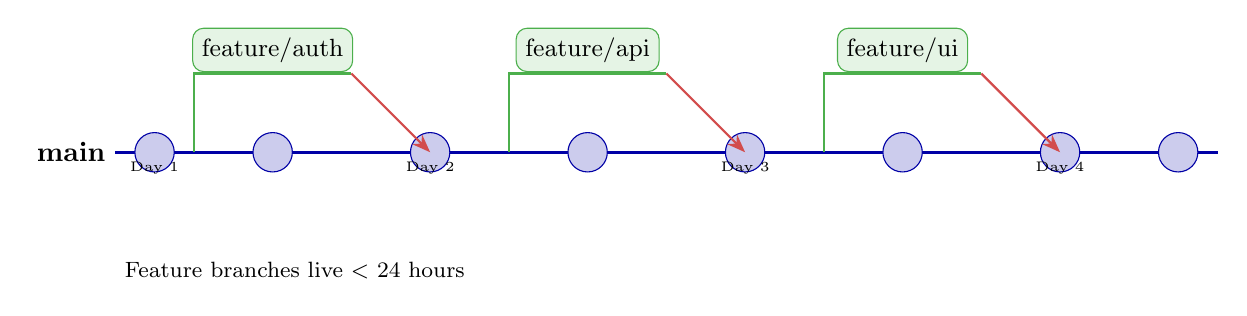
\begin{tikzpicture}[
  commit/.style={circle, draw=BlueKey, fill=BlueKey!20, minimum size=0.5cm},
  branch/.style={rectangle, rounded corners, draw=GreenExample!70, fill=GreenExample!10, minimum height=0.5cm, font=\small},
  mainline/.style={very thick, BlueKey},
  featureline/.style={thick, GreenExample!70},
  mergearrow/.style={-Stealth, thick, RedResult!70}
]

% Main branch
\draw[mainline] (0,0) -- (14,0);
\node[left] at (0,0) {\textbf{main}};

% Commits on main
\foreach \x in {0.5,2,4,6,8,10,12,13.5} {
  \node[commit] at (\x,0) {};
}

% Feature branch 1
\draw[featureline] (1,0) -- (1,1) -- (3,1);
\draw[mergearrow] (3,1) -- (4,0);
\node[branch] at (2,1.3) {feature/auth};

% Feature branch 2
\draw[featureline] (5,0) -- (5,1) -- (7,1);
\draw[mergearrow] (7,1) -- (8,0);
\node[branch] at (6,1.3) {feature/api};

% Feature branch 3
\draw[featureline] (9,0) -- (9,1) -- (11,1);
\draw[mergearrow] (11,1) -- (12,0);
\node[branch] at (10,1.3) {feature/ui};

% Time labels
\node[below] at (0.5,0) {\tiny Day 1};
\node[below] at (4,0) {\tiny Day 2};
\node[below] at (8,0) {\tiny Day 3};
\node[below] at (12,0) {\tiny Day 4};

% Legend
\node[right, font=\footnotesize] at (0,-1.5) {Feature branches live $<$ 24 hours};

\end{tikzpicture}
\end{center}

\clearpage
\paragraph{Key Principles}

\begin{enumerate}
  \item \textbf{Short-Lived Feature Branches}: Branches should be merged within 24 hours
  \item \textbf{Feature Flags}: Use feature flags to hide incomplete features
  \item \textbf{Continuous Integration}: Merge to trunk multiple times per day
  \item \textbf{Release from Trunk}: Production deployments come directly from the main branch
\end{enumerate}

\begin{lstlisting}[language=yaml,caption={GitHub Actions Workflow for Trunk-Based Development}]
name: Trunk-Based CI/CD

on:
  push:
    branches: [main]
  pull_request:
    branches: [main]

jobs:
  validate:
    runs-on: ubuntu-latest
    steps:
      - uses: actions/checkout@v4
        with:
          fetch-depth: 0

      - name: Check Branch Age
        if: github.event_name == 'pull_request'
        run: |
          BRANCH_AGE=$(git log -1 --format=%ct origin/main..HEAD)
          CURRENT_TIME=$(date +%s)
          AGE_HOURS=$(( (CURRENT_TIME - BRANCH_AGE) / 3600 ))
          if [ $AGE_HOURS -gt 24 ]; then
            echo "::warning::Branch is older than 24 hours. Consider rebasing."
          fi

      - name: Verify Linear History
        run: |
          if ! git log --oneline --merges origin/main..HEAD | grep -q .; then
            echo "Linear history maintained"
          else
            echo "::error::Merge commits detected. Use rebase instead."
            exit 1
          fi
\end{lstlisting}

\subsubsection{GitFlow for Scheduled Releases}

GitFlow is appropriate for teams with scheduled release cycles and multiple supported versions.

\begin{center}
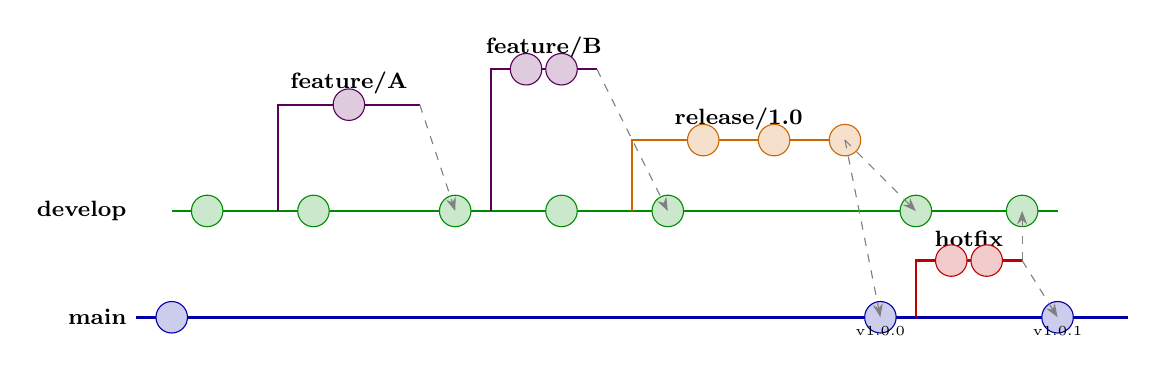
\begin{tikzpicture}[
  scale=0.9,
  commit/.style={circle, draw=BlueKey, fill=BlueKey!20, minimum size=0.4cm},
  commitrel/.style={circle, draw=OrangeAction, fill=OrangeAction!20, minimum size=0.4cm},
  commitdev/.style={circle, draw=GreenExample, fill=GreenExample!20, minimum size=0.4cm},
  commitfeat/.style={circle, draw=PurpleNote, fill=PurpleNote!20, minimum size=0.4cm},
  commitfix/.style={circle, draw=RedResult, fill=RedResult!20, minimum size=0.4cm},
  branchlabel/.style={font=\footnotesize\bfseries},
  mainline/.style={very thick, BlueKey},
  devline/.style={thick, GreenExample},
  relline/.style={thick, OrangeAction},
  featline/.style={thick, PurpleNote},
  fixline/.style={thick, RedResult},
  mergearrow/.style={-Stealth, dashed, gray}
]

% Main branch (bottom)
\draw[mainline] (0,0) -- (14,0);
\node[branchlabel, left] at (0,0) {main};

% Develop branch
\draw[devline] (0.5,1.5) -- (13,1.5);
\node[branchlabel, left] at (0,1.5) {develop};

% Release branch
\draw[relline] (7,1.5) -- (7,2.5) -- (10,2.5);
\node[branchlabel] at (8.5,2.8) {release/1.0};

% Feature branches
\draw[featline] (2,1.5) -- (2,3) -- (4,3);
\draw[featline] (5,1.5) -- (5,3.5) -- (6.5,3.5);
\node[branchlabel] at (3,3.3) {feature/A};
\node[branchlabel] at (5.75,3.8) {feature/B};

% Hotfix branch
\draw[fixline] (11,0) -- (11,0.8) -- (12.5,0.8);
\node[branchlabel] at (11.75,1.1) {hotfix};

% Commits on main
\node[commit] at (0.5,0) {};
\node[commit] at (10.5,0) {};
\node[commit] at (13,0) {};

% Commits on develop
\foreach \x in {1,2.5,4.5,6,7.5,11,12.5} {
  \node[commitdev] at (\x,1.5) {};
}

% Commits on release
\foreach \x in {8,9,10} {
  \node[commitrel] at (\x,2.5) {};
}

% Commits on features
\node[commitfeat] at (3,3) {};
\node[commitfeat] at (5.5,3.5) {};
\node[commitfeat] at (6,3.5) {};

% Commits on hotfix
\node[commitfix] at (11.5,0.8) {};
\node[commitfix] at (12,0.8) {};

% Merge arrows
\draw[mergearrow] (4,3) -- (4.5,1.5);
\draw[mergearrow] (6.5,3.5) -- (7.5,1.5);
\draw[mergearrow] (10,2.5) -- (10.5,0);
\draw[mergearrow] (10,2.5) -- (11,1.5);
\draw[mergearrow] (12.5,0.8) -- (13,0);
\draw[mergearrow] (12.5,0.8) -- (12.5,1.5);

% Tags
\node[below, font=\tiny] at (10.5,0) {v1.0.0};
\node[below, font=\tiny] at (13,0) {v1.0.1};

\end{tikzpicture}
\end{center}

\begin{lstlisting}[language=yaml,caption={GitFlow Branch Naming Convention}]
# Branch naming patterns
branches:
  main:
    pattern: "^main$"
    protected: true
    deployment: production

  develop:
    pattern: "^develop$"
    protected: true
    deployment: staging

  feature:
    pattern: "^feature/[A-Z]+-[0-9]+-.+"
    example: "feature/PROJ-123-add-user-authentication"
    source: develop
    target: develop
    max_age_days: 14

  release:
    pattern: "^release/[0-9]+\\.[0-9]+\\.[0-9]+$"
    example: "release/1.2.0"
    source: develop
    target: [main, develop]

  hotfix:
    pattern: "^hotfix/[A-Z]+-[0-9]+-.+"
    example: "hotfix/PROJ-456-fix-critical-bug"
    source: main
    target: [main, develop]
    priority: high
\end{lstlisting}

\begin{warningbox}
GitFlow adds complexity and can slow down delivery if not managed properly. Reserve it for situations requiring multiple parallel release versions or strict release scheduling. For most web applications, simpler strategies like Trunk-Based Development are more appropriate.
\end{warningbox}

\subsection{Metrics and Compliance}

\subsubsection{Key Metrics for SCM Gates}

\begin{table}[H]
\centering
\caption{Source Code Management Metrics}
\rowcolors{2}{TableAlt}{white}
\begin{tabular}{L{4cm}L{3cm}L{2.5cm}L{3.5cm}}
\toprule
\rowcolor{TableHeader}
\textbf{Metric} & \textbf{Target} & \textbf{Warning} & \textbf{Measurement} \\
\midrule
Branch Age & $<$ 24 hours & $>$ 48 hours & Time since branch creation \\
PR Review Time & $<$ 4 hours & $>$ 24 hours & Time to first review \\
PR Merge Time & $<$ 8 hours & $>$ 48 hours & Time from open to merge \\
Review Approval Rate & $>$ 95\% & $<$ 90\% & PRs approved vs rejected \\
Commit Frequency & $>$ 1/day/dev & $<$ 1/week/dev & Commits per developer \\
Integration Frequency & $>$ 1/day & $<$ 1/week & Merges to main \\
Rollback Rate & $<$ 5\% & $>$ 10\% & Reverted deployments \\
\bottomrule
\end{tabular}
\end{table}

\newpage

%==================================================================
% SECTION 2: BUILD AND QUALITY GATES
%==================================================================
\section{Build and Quality Gates}

\begin{gatebox}
\gates{\gatepill{Static Analysis}\ \gatepill{80\% Code Coverage}}
\end{gatebox}

Build and Quality Gates ensure that every code change meets established quality standards before it can progress through the pipeline. These gates enforce automated checks that would be impractical to perform manually.

\subsection{Gate 3: Static Analysis}

\subsubsection{Overview}

Static analysis examines source code without executing it, identifying potential bugs, security vulnerabilities, code smells, and style violations. This gate prevents known categories of defects from entering the codebase.

\subsubsection{Static Analysis Tool Categories}

\begin{table}[H]
\centering
\caption{Static Analysis Tool Categories and Examples}
\rowcolors{2}{TableAlt}{white}
\begin{tabular}{L{3cm}L{4cm}L{6cm}}
\toprule
\rowcolor{TableHeader}
\textbf{Category} & \textbf{Tools} & \textbf{Purpose} \\
\midrule
Linters & ESLint, Pylint, RuboCop, golangci-lint & Style enforcement, basic error detection \\
Type Checkers & TypeScript, mypy, Flow & Type safety verification \\
Security Scanners & Semgrep, Bandit, Brakeman & Security vulnerability detection \\
Code Quality & SonarQube, CodeClimate & Comprehensive quality metrics \\
Complexity & Lizard, radon & Cyclomatic complexity analysis \\
Duplication & CPD, jscpd & Duplicate code detection \\
\bottomrule
\end{tabular}
\end{table}

\clearpage
\subsubsection{SonarQube Configuration}

SonarQube provides comprehensive code quality analysis across multiple dimensions.

\begin{lstlisting}[caption={sonar-project.properties Configuration}]
# Project identification
sonar.projectKey=mycompany_myproject
sonar.projectName=My Project
sonar.projectVersion=1.0

# Source configuration
sonar.sources=src
sonar.tests=tests
sonar.exclusions=**/node_modules/**,**/vendor/**,**/*.test.js

# Language-specific settings
sonar.javascript.lcov.reportPaths=coverage/lcov.info
sonar.python.coverage.reportPaths=coverage.xml
sonar.java.binaries=target/classes

# Quality gate settings
sonar.qualitygate.wait=true
sonar.qualitygate.timeout=300

# Issue severity thresholds
sonar.issue.ignore.multicriteria=e1,e2
sonar.issue.ignore.multicriteria.e1.ruleKey=javascript:S1135
sonar.issue.ignore.multicriteria.e1.resourceKey=**/*.spec.js
sonar.issue.ignore.multicriteria.e2.ruleKey=python:S1135
sonar.issue.ignore.multicriteria.e2.resourceKey=**/test_*.py

# Branch analysis
sonar.branch.name=${BRANCH_NAME}
sonar.branch.target=main
\end{lstlisting}

\clearpage
\subsubsection{Quality Gate Definition}

\begin{lstlisting}[language=yaml,caption={SonarQube Quality Gate Configuration}]
quality_gate:
  name: "Production Quality Gate"
  conditions:
    # Reliability
    - metric: new_bugs
      operator: GREATER_THAN
      error: 0

    - metric: new_reliability_rating
      operator: GREATER_THAN
      error: 1  # Must be A rating

    # Security
    - metric: new_vulnerabilities
      operator: GREATER_THAN
      error: 0

    - metric: new_security_rating
      operator: GREATER_THAN
      error: 1  # Must be A rating

    - metric: new_security_hotspots_reviewed
      operator: LESS_THAN
      error: 100  # All hotspots must be reviewed

    # Maintainability
    - metric: new_code_smells
      operator: GREATER_THAN
      error: 10  # Allow up to 10 new code smells

    - metric: new_maintainability_rating
      operator: GREATER_THAN
      error: 1  # Must be A rating

    - metric: new_technical_debt_ratio
      operator: GREATER_THAN
      error: 5  # Max 5% technical debt ratio

    # Coverage
    - metric: new_coverage
      operator: LESS_THAN
      error: 80  # Minimum 80% coverage on new code

    - metric: new_line_coverage
      operator: LESS_THAN
      error: 80

    # Duplication
    - metric: new_duplicated_lines_density
      operator: GREATER_THAN
      error: 3  # Max 3% duplication
\end{lstlisting}

\clearpage
\subsubsection{Multi-Language Linting Configuration}

\begin{lstlisting}[language=yaml,caption={GitHub Actions Multi-Language Linting Workflow}]
name: Static Analysis

on:
  pull_request:
    branches: [main, develop]

jobs:
  lint-javascript:
    runs-on: ubuntu-latest
    steps:
      - uses: actions/checkout@v4

      - name: Setup Node.js
        uses: actions/setup-node@v4
        with:
          node-version: '20'
          cache: 'npm'

      - run: npm ci

      - name: Run ESLint
        run: |
          npx eslint . \
            --format json \
            --output-file eslint-report.json \
            --max-warnings 0

      - name: Upload ESLint Report
        uses: actions/upload-artifact@v4
        with:
          name: eslint-report
          path: eslint-report.json

  lint-python:
    runs-on: ubuntu-latest
    steps:
      - uses: actions/checkout@v4

      - name: Setup Python
        uses: actions/setup-python@v5
        with:
          python-version: '3.12'

      - name: Install dependencies
        run: |
          pip install pylint mypy ruff bandit

      - name: Run Ruff (fast linting)
        run: ruff check . --output-format=json > ruff-report.json

      - name: Run Pylint
        run: |
          pylint src/ \
            --output-format=json \
            --fail-under=8.0 \
            > pylint-report.json || true

      - name: Run mypy (type checking)
        run: mypy src/ --strict --ignore-missing-imports

      - name: Run Bandit (security)
        run: bandit -r src/ -f json -o bandit-report.json

  lint-go:
    runs-on: ubuntu-latest
    steps:
      - uses: actions/checkout@v4

      - name: Setup Go
        uses: actions/setup-go@v5
        with:
          go-version: '1.22'

      - name: Run golangci-lint
        uses: golangci/golangci-lint-action@v4
        with:
          version: latest
          args: --timeout=5m

  sonarqube:
    needs: [lint-javascript, lint-python, lint-go]
    runs-on: ubuntu-latest
    steps:
      - uses: actions/checkout@v4
        with:
          fetch-depth: 0

      - name: Download all reports
        uses: actions/download-artifact@v4

      - name: SonarQube Scan
        uses: sonarsource/sonarqube-scan-action@master
        env:
          SONAR_TOKEN: ${{ secrets.SONAR_TOKEN }}
          SONAR_HOST_URL: ${{ secrets.SONAR_HOST_URL }}

      - name: SonarQube Quality Gate
        uses: sonarsource/sonarqube-quality-gate-action@master
        timeout-minutes: 5
        env:
          SONAR_TOKEN: ${{ secrets.SONAR_TOKEN }}
\end{lstlisting}

\clearpage
\subsection{Gate 4: 80\% Code Coverage}

\subsubsection{Overview}

Code coverage measures the percentage of code executed during automated testing. The 80\% threshold represents an industry-standard balance between thoroughness and practicality.

\subsubsection{Coverage Types}

\begin{table}[H]
\centering
\caption{Types of Code Coverage}
\rowcolors{2}{TableAlt}{white}
\begin{tabular}{L{3cm}L{4.5cm}L{5.5cm}}
\toprule
\rowcolor{TableHeader}
\textbf{Type} & \textbf{Description} & \textbf{Target} \\
\midrule
Line Coverage & Percentage of lines executed & Primary metric, $\geq$ 80\% \\
Branch Coverage & Percentage of branches taken & Critical for conditionals, $\geq$ 75\% \\
Function Coverage & Percentage of functions called & Should approach 100\% \\
Statement Coverage & Percentage of statements run & Similar to line coverage \\
Condition Coverage & Each boolean evaluated both ways & Important for complex logic \\
MC/DC Coverage & Modified condition/decision & Required for safety-critical code \\
\bottomrule
\end{tabular}
\end{table}

\clearpage
\subsubsection{Coverage Configuration Examples}

\begin{lstlisting}[caption={Jest Coverage Configuration (jest.config.js)}]
module.exports = {
  collectCoverage: true,
  collectCoverageFrom: [
    'src/**/*.{js,jsx,ts,tsx}',
    '!src/**/*.d.ts',
    '!src/**/*.stories.{js,jsx,ts,tsx}',
    '!src/**/*.test.{js,jsx,ts,tsx}',
    '!src/**/index.{js,ts}',
    '!src/mocks/**'
  ],
  coverageDirectory: 'coverage',
  coverageReporters: ['text', 'lcov', 'html', 'cobertura'],
  coverageThreshold: {
    global: {
      branches: 75,
      functions: 80,
      lines: 80,
      statements: 80
    },
    // Stricter thresholds for critical paths
    './src/auth/**/*.ts': {
      branches: 90,
      functions: 95,
      lines: 90,
      statements: 90
    },
    './src/payment/**/*.ts': {
      branches: 95,
      functions: 100,
      lines: 95,
      statements: 95
    }
  },
  testMatch: [
    '**/__tests__/**/*.[jt]s?(x)',
    '**/?(*.)+(spec|test).[jt]s?(x)'
  ],
  testPathIgnorePatterns: [
    '/node_modules/',
    '/dist/'
  ]
};
\end{lstlisting}

\clearpage
\begin{lstlisting}[caption={pytest Coverage Configuration (pyproject.toml)}]
[tool.pytest.ini_options]
testpaths = ["tests"]
python_files = ["test_*.py", "*_test.py"]
python_functions = ["test_*"]
addopts = [
    "-v",
    "--tb=short",
    "--strict-markers",
    "--cov=src",
    "--cov-report=term-missing",
    "--cov-report=html:coverage_html",
    "--cov-report=xml:coverage.xml",
    "--cov-fail-under=80",
    "--cov-branch"
]

[tool.coverage.run]
branch = true
source = ["src"]
omit = [
    "*/tests/*",
    "*/__pycache__/*",
    "*/migrations/*",
    "*/.venv/*"
]

[tool.coverage.report]
exclude_lines = [
    "pragma: no cover",
    "def __repr__",
    "raise NotImplementedError",
    "if __name__ == .__main__.:",
    "if TYPE_CHECKING:",
    "@abstractmethod"
]
fail_under = 80
show_missing = true
precision = 2

[tool.coverage.html]
directory = "coverage_html"
\end{lstlisting}

\clearpage
\begin{lstlisting}[caption={JaCoCo Configuration for Java (pom.xml excerpt)}]
<plugin>
  <groupId>org.jacoco</groupId>
  <artifactId>jacoco-maven-plugin</artifactId>
  <version>0.8.11</version>
  <executions>
    <execution>
      <id>prepare-agent</id>
      <goals>
        <goal>prepare-agent</goal>
      </goals>
    </execution>
    <execution>
      <id>report</id>
      <phase>test</phase>
      <goals>
        <goal>report</goal>
      </goals>
    </execution>
    <execution>
      <id>check</id>
      <goals>
        <goal>check</goal>
      </goals>
      <configuration>
        <rules>
          <rule>
            <element>BUNDLE</element>
            <limits>
              <limit>
                <counter>LINE</counter>
                <value>COVEREDRATIO</value>
                <minimum>0.80</minimum>
              </limit>
              <limit>
                <counter>BRANCH</counter>
                <value>COVEREDRATIO</value>
                <minimum>0.75</minimum>
              </limit>
            </limits>
          </rule>
          <rule>
            <element>CLASS</element>
            <limits>
              <limit>
                <counter>LINE</counter>
                <value>COVEREDRATIO</value>
                <minimum>0.70</minimum>
              </limit>
            </limits>
            <excludes>
              <exclude>*Exception</exclude>
              <exclude>*Config</exclude>
            </excludes>
          </rule>
        </rules>
      </configuration>
    </execution>
  </executions>
</plugin>
\end{lstlisting}

\clearpage
\subsubsection{Coverage Enforcement in CI/CD}

\begin{lstlisting}[language=yaml,caption={GitHub Actions Coverage Enforcement}]
name: Test Coverage

on:
  pull_request:
    branches: [main]

jobs:
  coverage:
    runs-on: ubuntu-latest
    steps:
      - uses: actions/checkout@v4

      - name: Setup Node.js
        uses: actions/setup-node@v4
        with:
          node-version: '20'
          cache: 'npm'

      - run: npm ci

      - name: Run Tests with Coverage
        run: npm run test:coverage

      - name: Check Coverage Thresholds
        run: |
          COVERAGE=$(cat coverage/coverage-summary.json | \
            jq '.total.lines.pct')
          echo "Line coverage: ${COVERAGE}%"

          if (( $(echo "$COVERAGE < 80" | bc -l) )); then
            echo "::error::Coverage ${COVERAGE}% is below 80% threshold"
            exit 1
          fi

      - name: Upload Coverage to Codecov
        uses: codecov/codecov-action@v4
        with:
          token: ${{ secrets.CODECOV_TOKEN }}
          files: ./coverage/lcov.info
          fail_ci_if_error: true
          verbose: true

      - name: Comment Coverage on PR
        uses: actions/github-script@v7
        with:
          script: |
            const fs = require('fs');
            const summary = JSON.parse(
              fs.readFileSync('coverage/coverage-summary.json')
            );

            const body = `## Coverage Report

            | Metric | Coverage |
            |--------|----------|
            | Lines | ${summary.total.lines.pct}% |
            | Branches | ${summary.total.branches.pct}% |
            | Functions | ${summary.total.functions.pct}% |
            | Statements | ${summary.total.statements.pct}% |`;

            github.rest.issues.createComment({
              issue_number: context.issue.number,
              owner: context.repo.owner,
              repo: context.repo.repo,
              body: body
            });
\end{lstlisting}

\begin{tipbox}
Coverage metrics should be enforced differently for new code versus existing code. Require 80\%+ coverage on new code while gradually improving legacy code coverage. Use SonarQube's ``New Code'' analysis to enforce stricter standards on changes.
\end{tipbox}

\begin{warningbox}
High coverage does not guarantee high-quality tests. A codebase can achieve 100\% coverage with tests that have no assertions. Always combine coverage metrics with mutation testing (using tools like Stryker or PIT) to verify test effectiveness.
\end{warningbox}

\newpage

%==================================================================
% SECTION 3: SECURITY SCANNING
%==================================================================
\section{Security Scanning}

\begin{gatebox}
\gates{\gatepill{Vulnerability Scan}\ \gatepill{Open Source Scan}}
\end{gatebox}

Security scanning gates integrate security into the development lifecycle, implementing the ``shift left'' security philosophy. These gates automatically detect vulnerabilities before they reach production.

\subsection{Gate 5: Vulnerability Scan}

\subsubsection{Security Scanning Categories}

\begin{table}[H]
\centering
\caption{Security Scanning Types}
\rowcolors{2}{TableAlt}{white}
\begin{tabular}{L{2.2cm}L{3.5cm}L{3.5cm}L{3.8cm}}
\toprule
\rowcolor{TableHeader}
\textbf{Type} & \textbf{What It Scans} & \textbf{Tools} & \textbf{When to Run} \\
\midrule
SAST & Source code patterns & Semgrep, CodeQL, Checkmarx & Every commit \\
SCA & Dependencies & Snyk, Dependabot, OWASP DC & Every build \\
DAST & Running application & OWASP ZAP, Burp Suite & Post-deployment \\
Container & Container images & Trivy, Grype, Clair & Image build \\
IaC & Infrastructure code & Checkov, tfsec, KICS & Infrastructure changes \\
Secrets & Hardcoded secrets & Gitleaks, TruffleHog & Pre-commit, CI \\
\bottomrule
\end{tabular}
\end{table}

\clearpage
\subsubsection{SAST Implementation with Semgrep}

\begin{lstlisting}[language=yaml,caption={Semgrep Configuration (.semgrep.yml)}]
rules:
  # SQL Injection Detection
  - id: sql-injection
    patterns:
      - pattern-either:
          - pattern: |
              $QUERY = "..." + $USER_INPUT + "..."
              $DB.execute($QUERY)
          - pattern: |
              $DB.execute(f"...{$USER_INPUT}...")
    message: "Potential SQL injection vulnerability"
    severity: ERROR
    languages: [python, javascript]
    metadata:
      cwe: "CWE-89"
      owasp: "A03:2021"

  # Hardcoded Secrets
  - id: hardcoded-secret
    pattern-regex: |
      (?i)(password|secret|api_key|token)\s*=\s*['\"][^'\"]{8,}['\"]
    message: "Potential hardcoded secret detected"
    severity: ERROR
    languages: [generic]
    metadata:
      cwe: "CWE-798"

  # Insecure Deserialization
  - id: insecure-pickle
    patterns:
      - pattern: pickle.loads($DATA)
      - pattern-not-inside: |
          if is_trusted($DATA):
              ...
    message: "Unsafe pickle deserialization"
    severity: ERROR
    languages: [python]
    metadata:
      cwe: "CWE-502"

  # Path Traversal
  - id: path-traversal
    patterns:
      - pattern: open($USER_INPUT)
      - pattern-not: open(os.path.join($SAFE_DIR, os.path.basename($USER_INPUT)))
    message: "Potential path traversal vulnerability"
    severity: WARNING
    languages: [python]
    metadata:
      cwe: "CWE-22"
\end{lstlisting}

\clearpage
\subsubsection{Container Image Scanning with Trivy}

\begin{lstlisting}[language=yaml,caption={Trivy Container Scanning Workflow}]
name: Container Security Scan

on:
  push:
    paths:
      - 'Dockerfile*'
      - '.dockerignore'
      - 'docker-compose*.yml'

jobs:
  scan:
    runs-on: ubuntu-latest
    steps:
      - uses: actions/checkout@v4

      - name: Build Image
        run: docker build -t myapp:${{ github.sha }} .

      - name: Run Trivy Vulnerability Scanner
        uses: aquasecurity/trivy-action@master
        with:
          image-ref: 'myapp:${{ github.sha }}'
          format: 'sarif'
          output: 'trivy-results.sarif'
          severity: 'CRITICAL,HIGH'
          vuln-type: 'os,library'
          ignore-unfixed: true

      - name: Upload Trivy Scan Results
        uses: github/codeql-action/upload-sarif@v3
        with:
          sarif_file: 'trivy-results.sarif'

      - name: Fail on Critical Vulnerabilities
        uses: aquasecurity/trivy-action@master
        with:
          image-ref: 'myapp:${{ github.sha }}'
          exit-code: '1'
          severity: 'CRITICAL'
          vuln-type: 'os,library'
\end{lstlisting}

\clearpage
\subsubsection{Infrastructure as Code Scanning}

\begin{lstlisting}[language=yaml,caption={Checkov IaC Security Scanning}]
name: IaC Security Scan

on:
  pull_request:
    paths:
      - 'terraform/**'
      - 'kubernetes/**'
      - 'cloudformation/**'

jobs:
  checkov:
    runs-on: ubuntu-latest
    steps:
      - uses: actions/checkout@v4

      - name: Run Checkov
        uses: bridgecrewio/checkov-action@master
        with:
          directory: .
          framework: terraform,kubernetes,cloudformation
          output_format: sarif
          output_file_path: checkov-results.sarif
          soft_fail: false
          skip_check: CKV_AWS_18,CKV_AWS_21  # Document exceptions
          config_file: .checkov.yml

      - name: Upload Checkov Results
        uses: github/codeql-action/upload-sarif@v3
        with:
          sarif_file: checkov-results.sarif
\end{lstlisting}

\clearpage
\begin{lstlisting}[language=yaml,caption={Checkov Configuration (.checkov.yml)}]
# Checkov configuration
soft-fail: false
compact: true
framework:
  - terraform
  - kubernetes
  - dockerfile

# Severity thresholds
hard-fail-on:
  - CRITICAL
  - HIGH

# Skip specific checks with justification
skip-check:
  # Skip S3 versioning for ephemeral buckets
  - CKV_AWS_21:
      comment: "Ephemeral data bucket, versioning not required"
      resources:
        - aws_s3_bucket.temp_data

# Custom policies
external-checks-dir:
  - ./security/custom-policies

# Output configuration
output:
  - cli
  - sarif
  - json
\end{lstlisting}

\clearpage
\subsection{Gate 6: Open Source Scan}

\subsubsection{Software Composition Analysis}

Open Source Scan ensures that third-party dependencies do not introduce vulnerabilities or license compliance issues.

\begin{lstlisting}[language=yaml,caption={Snyk Configuration (.snyk)}]
# Snyk policy file
version: v1.25.0

# Ignore specific vulnerabilities with justification
ignore:
  SNYK-JS-LODASH-567746:
    - '*':
        reason: 'Not exploitable in our usage context'
        expires: '2025-01-01T00:00:00.000Z'
        created: '2024-01-01T00:00:00.000Z'

# Patch vulnerabilities when fixes aren't available
patch:
  SNYK-JS-HOEK-12345:
    - 'request > hawk > hoek':
        patched: '2024-06-01T00:00:00.000Z'

# Language-specific settings
language-settings:
  python:
    python-version: '3.12'

# License policies
license-policies:
  severity:
    - GPL-3.0: high
    - AGPL-3.0: critical
    - unlicensed: critical
  allow:
    - MIT
    - Apache-2.0
    - BSD-2-Clause
    - BSD-3-Clause
    - ISC
\end{lstlisting}

\clearpage
\subsubsection{OWASP Dependency-Check Configuration}

\begin{lstlisting}[language=yaml,caption={OWASP Dependency-Check GitHub Action}]
name: Dependency Security Scan

on:
  schedule:
    - cron: '0 6 * * *'  # Daily at 6 AM
  push:
    paths:
      - '**/package*.json'
      - '**/requirements*.txt'
      - '**/Pipfile*'
      - '**/pom.xml'
      - '**/build.gradle*'

jobs:
  dependency-check:
    runs-on: ubuntu-latest
    steps:
      - uses: actions/checkout@v4

      - name: Run OWASP Dependency-Check
        uses: dependency-check/Dependency-Check_Action@main
        with:
          project: 'MyProject'
          path: '.'
          format: 'ALL'
          args: >
            --failOnCVSS 7
            --enableRetired
            --enableExperimental
            --suppression ./dependency-suppression.xml

      - name: Upload Dependency-Check Report
        uses: actions/upload-artifact@v4
        with:
          name: dependency-check-report
          path: reports/

      - name: Publish to DefectDojo
        run: |
          curl -X POST "${{ secrets.DEFECTDOJO_URL }}/api/v2/import-scan/" \
            -H "Authorization: Token ${{ secrets.DEFECTDOJO_TOKEN }}" \
            -F "scan_type=Dependency Check Scan" \
            -F "file=@reports/dependency-check-report.xml" \
            -F "engagement=${{ secrets.DEFECTDOJO_ENGAGEMENT }}" \
            -F "verified=false" \
            -F "active=true"
\end{lstlisting}

\subsubsection{License Compliance Policy}

\begin{table}[H]
\centering
\caption{License Compliance Categories}
\rowcolors{2}{TableAlt}{white}
\begin{tabular}{L{3cm}L{4cm}L{6cm}}
\toprule
\rowcolor{TableHeader}
\textbf{Category} & \textbf{Licenses} & \textbf{Policy} \\
\midrule
Permissive & MIT, Apache 2.0, BSD & \good{Approved} for all use \\
Weak Copyleft & LGPL, MPL & \tip{Approved} with attribution \\
Strong Copyleft & GPL, AGPL & \warn{Restricted} - requires review \\
Proprietary & Commercial licenses & \warn{Restricted} - requires procurement \\
Unknown & No license specified & \warn{Blocked} - cannot use \\
\bottomrule
\end{tabular}
\end{table}

\begin{lstlisting}[language=yaml,caption={License Compliance Workflow}]
name: License Compliance

on:
  pull_request:
    paths:
      - '**/package*.json'
      - '**/requirements*.txt'
      - '**/go.mod'

jobs:
  license-check:
    runs-on: ubuntu-latest
    steps:
      - uses: actions/checkout@v4

      # Node.js license check
      - name: Check npm licenses
        run: |
          npx license-checker \
            --production \
            --json \
            --out licenses.json \
            --failOn "GPL-3.0;AGPL-3.0;UNLICENSED"

      # Python license check
      - name: Check pip licenses
        run: |
          pip install pip-licenses
          pip-licenses \
            --format=json \
            --output-file=python-licenses.json \
            --fail-on="GPL-3.0;AGPL-3.0"

      # Go license check
      - name: Check Go licenses
        run: |
          go install github.com/google/go-licenses@latest
          go-licenses check ./... \
            --disallowed_types=restricted,forbidden

      - name: Generate SBOM
        run: |
          npx @cyclonedx/cyclonedx-npm \
            --output-file sbom.json \
            --output-format json

      - name: Upload SBOM
        uses: actions/upload-artifact@v4
        with:
          name: sbom
          path: sbom.json
\end{lstlisting}

\newpage

%==================================================================
% SECTION 4: ARTIFACT MANAGEMENT
%==================================================================
\section{Artifact Management}

\begin{gatebox}
\gates{\gatepill{Artifact Version Control}}
\end{gatebox}

Artifact Management ensures that build outputs are properly versioned, stored, and retrievable for deployment to any environment.

\subsection{Gate 7: Artifact Version Control}

\subsubsection{Artifact Repository Architecture}

\begin{center}
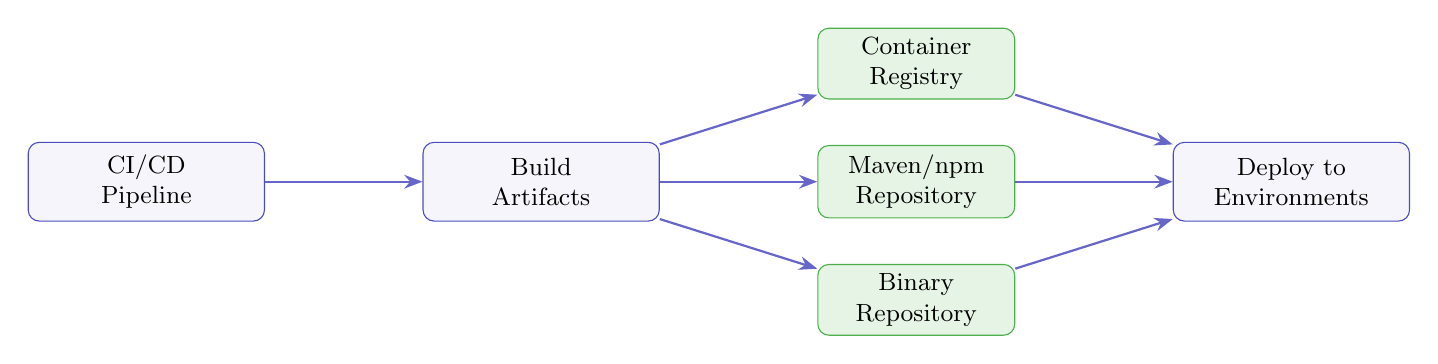
\begin{tikzpicture}[
  node distance=1.5cm,
  box/.style={rectangle, rounded corners, draw=BlueKey!70, fill=CardBg, minimum width=3cm, minimum height=1cm, align=center, font=\small},
  repo/.style={rectangle, rounded corners, draw=GreenExample!70, fill=GreenExample!10, minimum width=2.5cm, minimum height=0.8cm, align=center, font=\small},
  arrow/.style={-Stealth, thick, BlueKey!60}
]

% CI/CD Pipeline
\node[box] (ci) {CI/CD\\Pipeline};

% Artifact Types
\node[box, right=2cm of ci] (artifacts) {Build\\Artifacts};

% Repositories
\node[repo, right=2cm of artifacts, yshift=1.5cm] (docker) {Container\\Registry};
\node[repo, right=2cm of artifacts, yshift=0cm] (maven) {Maven/npm\\Repository};
\node[repo, right=2cm of artifacts, yshift=-1.5cm] (binary) {Binary\\Repository};

% Environments
\node[box, right=2cm of maven] (envs) {Deploy to\\Environments};

% Arrows
\draw[arrow] (ci) -- (artifacts);
\draw[arrow] (artifacts) -- (docker);
\draw[arrow] (artifacts) -- (maven);
\draw[arrow] (artifacts) -- (binary);
\draw[arrow] (docker) -- (envs);
\draw[arrow] (maven) -- (envs);
\draw[arrow] (binary) -- (envs);

\end{tikzpicture}
\end{center}

\clearpage
\subsubsection{Semantic Versioning Strategy}

\begin{lstlisting}[caption={Semantic Versioning with Semantic Release}]
// .releaserc.json
{
  "branches": ["main", {"name": "beta", "prerelease": true}],
  "plugins": [
    ["@semantic-release/commit-analyzer", {
      "preset": "conventionalcommits",
      "releaseRules": [
        {"type": "feat", "release": "minor"},
        {"type": "fix", "release": "patch"},
        {"type": "perf", "release": "patch"},
        {"breaking": true, "release": "major"},
        {"type": "docs", "release": false},
        {"type": "style", "release": false},
        {"type": "refactor", "release": "patch"},
        {"type": "test", "release": false},
        {"type": "ci", "release": false}
      ]
    }],
    "@semantic-release/release-notes-generator",
    "@semantic-release/changelog",
    ["@semantic-release/npm", {
      "npmPublish": true
    }],
    ["@semantic-release/git", {
      "assets": ["package.json", "CHANGELOG.md"],
      "message": "chore(release): ${nextRelease.version}"
    }],
    "@semantic-release/github"
  ]
}
\end{lstlisting}

\clearpage
\subsubsection{Container Image Tagging Strategy}

\begin{lstlisting}[language=yaml,caption={Docker Image Build and Push Workflow}]
name: Build and Push Container

on:
  push:
    branches: [main]
    tags: ['v*']

env:
  REGISTRY: ghcr.io
  IMAGE_NAME: ${{ github.repository }}

jobs:
  build:
    runs-on: ubuntu-latest
    permissions:
      contents: read
      packages: write

    steps:
      - uses: actions/checkout@v4

      - name: Set up Docker Buildx
        uses: docker/setup-buildx-action@v3

      - name: Log in to Container Registry
        uses: docker/login-action@v3
        with:
          registry: ${{ env.REGISTRY }}
          username: ${{ github.actor }}
          password: ${{ secrets.GITHUB_TOKEN }}

      - name: Extract metadata
        id: meta
        uses: docker/metadata-action@v5
        with:
          images: ${{ env.REGISTRY }}/${{ env.IMAGE_NAME }}
          tags: |
            # Branch name
            type=ref,event=branch
            # Git short SHA
            type=sha,prefix=sha-
            # Semantic version from tag
            type=semver,pattern={{version}}
            type=semver,pattern={{major}}.{{minor}}
            type=semver,pattern={{major}}
            # Latest tag for main branch
            type=raw,value=latest,enable=${{ github.ref == 'refs/heads/main' }}
            # Build timestamp
            type=raw,value={{date 'YYYYMMDD-HHmmss'}}

      - name: Build and push
        uses: docker/build-push-action@v5
        with:
          context: .
          push: true
          tags: ${{ steps.meta.outputs.tags }}
          labels: ${{ steps.meta.outputs.labels }}
          cache-from: type=gha
          cache-to: type=gha,mode=max
          build-args: |
            VERSION=${{ github.ref_name }}
            COMMIT=${{ github.sha }}
            BUILD_DATE=${{ github.event.head_commit.timestamp }}

      - name: Sign the container image
        run: |
          cosign sign --yes \
            ${{ env.REGISTRY }}/${{ env.IMAGE_NAME }}@${{ steps.build.outputs.digest }}
        env:
          COSIGN_EXPERIMENTAL: 1
\end{lstlisting}

\clearpage
\subsubsection{Artifact Integrity Verification}

\begin{lstlisting}[language=yaml,caption={Artifact Signing and Verification}]
name: Artifact Integrity

jobs:
  sign:
    runs-on: ubuntu-latest
    steps:
      - name: Generate SBOM
        uses: anchore/sbom-action@v0
        with:
          path: .
          format: cyclonedx-json
          output-file: sbom.json

      - name: Sign SBOM with Sigstore
        run: |
          cosign sign-blob \
            --yes \
            --bundle sbom.bundle \
            sbom.json

      - name: Attest SBOM to image
        run: |
          cosign attest \
            --yes \
            --predicate sbom.json \
            --type cyclonedx \
            ${{ env.REGISTRY }}/${{ env.IMAGE_NAME }}@${{ needs.build.outputs.digest }}

      - name: Generate SLSA Provenance
        uses: slsa-framework/slsa-github-generator/.github/workflows/generator_container_slsa3.yml@v1.9.0
        with:
          image: ${{ env.REGISTRY }}/${{ env.IMAGE_NAME }}
          digest: ${{ needs.build.outputs.digest }}

  verify:
    needs: sign
    runs-on: ubuntu-latest
    steps:
      - name: Verify image signature
        run: |
          cosign verify \
            --certificate-identity-regexp ".*@mycompany.com" \
            --certificate-oidc-issuer https://token.actions.githubusercontent.com \
            ${{ env.REGISTRY }}/${{ env.IMAGE_NAME }}:latest

      - name: Verify SBOM attestation
        run: |
          cosign verify-attestation \
            --type cyclonedx \
            --certificate-identity-regexp ".*@mycompany.com" \
            --certificate-oidc-issuer https://token.actions.githubusercontent.com \
            ${{ env.REGISTRY }}/${{ env.IMAGE_NAME }}@${{ needs.build.outputs.digest }}
\end{lstlisting}

\newpage

%==================================================================
% SECTION 5: INFRASTRUCTURE PROVISIONING
%==================================================================
\section{Infrastructure Provisioning}

\begin{gatebox}
\gates{\gatepill{Automatic Provision}\ \gatepill{Immutable Servers}}
\end{gatebox}

Infrastructure Provisioning gates ensure that deployment environments are created automatically, consistently, and without manual intervention.

\subsection{Gate 8: Automatic Provision}

\subsubsection{Infrastructure as Code with Terraform}

\begin{lstlisting}[language=hcl,caption={Terraform Main Configuration (main.tf)}]
terraform {
  required_version = ">= 1.6.0"

  required_providers {
    aws = {
      source  = "hashicorp/aws"
      version = "~> 5.0"
    }
    kubernetes = {
      source  = "hashicorp/kubernetes"
      version = "~> 2.24"
    }
  }

  backend "s3" {
    bucket         = "mycompany-terraform-state"
    key            = "environments/production/terraform.tfstate"
    region         = "us-east-1"
    encrypt        = true
    dynamodb_table = "terraform-state-lock"
  }
}

# EKS Cluster
module "eks" {
  source  = "terraform-aws-modules/eks/aws"
  version = "~> 19.0"

  cluster_name    = var.cluster_name
  cluster_version = "1.28"

  vpc_id     = module.vpc.vpc_id
  subnet_ids = module.vpc.private_subnets

  cluster_endpoint_public_access = true

  eks_managed_node_groups = {
    general = {
      name           = "general-workloads"
      instance_types = ["m6i.large"]
      min_size       = 2
      max_size       = 10
      desired_size   = 3

      labels = {
        workload-type = "general"
      }

      tags = {
        Environment = var.environment
        Terraform   = "true"
      }
    }
  }

  # Enable IRSA
  enable_irsa = true

  tags = local.common_tags
}

# Application Load Balancer
module "alb" {
  source  = "terraform-aws-modules/alb/aws"
  version = "~> 9.0"

  name               = "${var.project_name}-alb"
  load_balancer_type = "application"
  vpc_id             = module.vpc.vpc_id
  subnets            = module.vpc.public_subnets
  security_groups    = [module.alb_sg.security_group_id]

  listeners = {
    https = {
      port            = 443
      protocol        = "HTTPS"
      certificate_arn = var.acm_certificate_arn

      forward = {
        target_group_key = "app"
      }
    }
  }

  target_groups = {
    app = {
      name_prefix      = "app-"
      protocol         = "HTTP"
      port             = 8080
      target_type      = "ip"

      health_check = {
        enabled             = true
        healthy_threshold   = 2
        unhealthy_threshold = 3
        interval            = 30
        path                = "/health"
        port                = "traffic-port"
      }
    }
  }

  tags = local.common_tags
}
\end{lstlisting}

\clearpage
\subsubsection{Terraform CI/CD Pipeline}

\begin{lstlisting}[language=yaml,caption={Terraform GitHub Actions Workflow}]
name: Terraform Infrastructure

on:
  push:
    branches: [main]
    paths:
      - 'terraform/**'
  pull_request:
    branches: [main]
    paths:
      - 'terraform/**'

env:
  TF_VERSION: '1.6.0'
  TF_WORKING_DIR: 'terraform/environments/production'

jobs:
  validate:
    runs-on: ubuntu-latest
    steps:
      - uses: actions/checkout@v4

      - name: Setup Terraform
        uses: hashicorp/setup-terraform@v3
        with:
          terraform_version: ${{ env.TF_VERSION }}

      - name: Terraform Format Check
        run: terraform fmt -check -recursive
        working-directory: terraform

      - name: Terraform Init
        run: terraform init -backend=false
        working-directory: ${{ env.TF_WORKING_DIR }}

      - name: Terraform Validate
        run: terraform validate
        working-directory: ${{ env.TF_WORKING_DIR }}

      - name: Run tfsec
        uses: aquasecurity/tfsec-action@v1.0.0
        with:
          working_directory: terraform
          soft_fail: false

      - name: Run Checkov
        uses: bridgecrewio/checkov-action@master
        with:
          directory: terraform
          framework: terraform

  plan:
    needs: validate
    runs-on: ubuntu-latest
    steps:
      - uses: actions/checkout@v4

      - name: Setup Terraform
        uses: hashicorp/setup-terraform@v3
        with:
          terraform_version: ${{ env.TF_VERSION }}

      - name: Configure AWS Credentials
        uses: aws-actions/configure-aws-credentials@v4
        with:
          role-to-assume: ${{ secrets.AWS_ROLE_ARN }}
          aws-region: us-east-1

      - name: Terraform Init
        run: terraform init
        working-directory: ${{ env.TF_WORKING_DIR }}

      - name: Terraform Plan
        id: plan
        run: |
          terraform plan \
            -input=false \
            -out=tfplan \
            -no-color
        working-directory: ${{ env.TF_WORKING_DIR }}

      - name: Upload Plan
        uses: actions/upload-artifact@v4
        with:
          name: terraform-plan
          path: ${{ env.TF_WORKING_DIR }}/tfplan

      - name: Post Plan to PR
        if: github.event_name == 'pull_request'
        uses: actions/github-script@v7
        with:
          script: |
            const output = `#### Terraform Plan
            \`\`\`
            ${{ steps.plan.outputs.stdout }}
            \`\`\``;
            github.rest.issues.createComment({
              issue_number: context.issue.number,
              owner: context.repo.owner,
              repo: context.repo.repo,
              body: output
            });

  apply:
    needs: plan
    if: github.ref == 'refs/heads/main' && github.event_name == 'push'
    runs-on: ubuntu-latest
    environment: production
    steps:
      - uses: actions/checkout@v4

      - name: Setup Terraform
        uses: hashicorp/setup-terraform@v3
        with:
          terraform_version: ${{ env.TF_VERSION }}

      - name: Configure AWS Credentials
        uses: aws-actions/configure-aws-credentials@v4
        with:
          role-to-assume: ${{ secrets.AWS_ROLE_ARN }}
          aws-region: us-east-1

      - name: Download Plan
        uses: actions/download-artifact@v4
        with:
          name: terraform-plan
          path: ${{ env.TF_WORKING_DIR }}

      - name: Terraform Init
        run: terraform init
        working-directory: ${{ env.TF_WORKING_DIR }}

      - name: Terraform Apply
        run: terraform apply -auto-approve tfplan
        working-directory: ${{ env.TF_WORKING_DIR }}
\end{lstlisting}

\clearpage
\subsection{Gate 9: Immutable Servers}

\subsubsection{Container Image Definition}

\begin{lstlisting}[caption={Production Dockerfile with Multi-Stage Build}]
# syntax=docker/dockerfile:1.6

# ============================================
# Stage 1: Dependencies
# ============================================
FROM node:20-alpine AS deps
WORKDIR /app

# Install dependencies only when needed
COPY package.json package-lock.json ./
RUN --mount=type=cache,target=/root/.npm \
    npm ci --only=production

# ============================================
# Stage 2: Builder
# ============================================
FROM node:20-alpine AS builder
WORKDIR /app

COPY --from=deps /app/node_modules ./node_modules
COPY . .

# Build application
RUN npm run build

# ============================================
# Stage 3: Production
# ============================================
FROM gcr.io/distroless/nodejs20-debian12 AS production

# Labels for container metadata
LABEL org.opencontainers.image.title="My Application" \
      org.opencontainers.image.description="Production application" \
      org.opencontainers.image.vendor="MyCompany" \
      org.opencontainers.image.source="https://github.com/mycompany/myapp"

WORKDIR /app

# Copy only production artifacts
COPY --from=builder /app/dist ./dist
COPY --from=builder /app/node_modules ./node_modules
COPY --from=builder /app/package.json ./

# Set environment
ENV NODE_ENV=production \
    PORT=8080

# Non-root user (distroless uses nonroot by default)
USER nonroot

# Health check
HEALTHCHECK --interval=30s --timeout=3s --start-period=5s --retries=3 \
    CMD ["/nodejs/bin/node", "-e", "require('http').get('http://localhost:8080/health')"]

EXPOSE 8080

CMD ["dist/server.js"]
\end{lstlisting}

\clearpage
\subsubsection{AMI Building with Packer}

\begin{lstlisting}[language=hcl,caption={Packer Configuration for Immutable AMI}]
packer {
  required_plugins {
    amazon = {
      version = ">= 1.2.0"
      source  = "github.com/hashicorp/amazon"
    }
    ansible = {
      version = ">= 1.1.0"
      source  = "github.com/hashicorp/ansible"
    }
  }
}

source "amazon-ebs" "app" {
  ami_name      = "myapp-${var.version}-{{timestamp}}"
  instance_type = "t3.medium"
  region        = var.aws_region

  source_ami_filter {
    filters = {
      name                = "ubuntu/images/hvm-ssd/ubuntu-jammy-22.04-amd64-server-*"
      root-device-type    = "ebs"
      virtualization-type = "hvm"
    }
    owners      = ["099720109477"]  # Canonical
    most_recent = true
  }

  ssh_username = "ubuntu"

  launch_block_device_mappings {
    device_name           = "/dev/sda1"
    volume_size           = 30
    volume_type           = "gp3"
    encrypted             = true
    delete_on_termination = true
  }

  tags = {
    Name        = "myapp-${var.version}"
    Version     = var.version
    BuildDate   = timestamp()
    GitCommit   = var.git_commit
    Environment = var.environment
  }
}

build {
  sources = ["source.amazon-ebs.app"]

  provisioner "shell" {
    inline = [
      "sudo apt-get update",
      "sudo apt-get install -y python3 python3-pip"
    ]
  }

  provisioner "ansible" {
    playbook_file = "ansible/playbook.yml"
    extra_arguments = [
      "--extra-vars", "app_version=${var.version}"
    ]
  }

  provisioner "shell" {
    inline = [
      "sudo apt-get clean",
      "sudo rm -rf /var/lib/apt/lists/*",
      "sudo rm -rf /tmp/*"
    ]
  }

  post-processor "manifest" {
    output     = "manifest.json"
    strip_path = true
  }
}

variable "version" {
  type        = string
  description = "Application version"
}

variable "git_commit" {
  type        = string
  description = "Git commit SHA"
}

variable "aws_region" {
  type    = string
  default = "us-east-1"
}

variable "environment" {
  type    = string
  default = "production"
}
\end{lstlisting}

\newpage

%==================================================================
% SECTION 6: INTEGRATION AND PERFORMANCE TESTING
%==================================================================
\section{Integration and Performance Testing}

\begin{gatebox}
\gates{\gatepill{Integration Testing}\ \gatepill{Performance Testing}}
\end{gatebox}

Integration and Performance Testing gates verify that the application functions correctly in a production-like environment and meets performance requirements.

\subsection{Gate 10: Integration Testing}

\subsubsection{End-to-End Testing with Playwright}

\begin{lstlisting}[caption={Playwright Configuration (playwright.config.ts)}]
import { defineConfig, devices } from '@playwright/test';

export default defineConfig({
  testDir: './e2e',
  fullyParallel: true,
  forbidOnly: !!process.env.CI,
  retries: process.env.CI ? 2 : 0,
  workers: process.env.CI ? 4 : undefined,
  reporter: [
    ['html', { outputFolder: 'playwright-report' }],
    ['junit', { outputFile: 'test-results/junit.xml' }],
    ['json', { outputFile: 'test-results/results.json' }]
  ],

  use: {
    baseURL: process.env.BASE_URL || 'http://localhost:3000',
    trace: 'on-first-retry',
    screenshot: 'only-on-failure',
    video: 'retain-on-failure',
  },

  projects: [
    {
      name: 'chromium',
      use: { ...devices['Desktop Chrome'] },
    },
    {
      name: 'firefox',
      use: { ...devices['Desktop Firefox'] },
    },
    {
      name: 'webkit',
      use: { ...devices['Desktop Safari'] },
    },
    {
      name: 'mobile-chrome',
      use: { ...devices['Pixel 5'] },
    },
    {
      name: 'mobile-safari',
      use: { ...devices['iPhone 12'] },
    },
  ],

  webServer: process.env.CI ? undefined : {
    command: 'npm run start',
    url: 'http://localhost:3000',
    reuseExistingServer: !process.env.CI,
  },
});
\end{lstlisting}

\clearpage
\begin{lstlisting}[caption={Playwright E2E Test Example}]
import { test, expect } from '@playwright/test';

test.describe('User Authentication Flow', () => {
  test.beforeEach(async ({ page }) => {
    await page.goto('/');
  });

  test('should allow user to login', async ({ page }) => {
    // Navigate to login
    await page.click('[data-testid="login-button"]');

    // Fill credentials
    await page.fill('[data-testid="email-input"]', 'test@example.com');
    await page.fill('[data-testid="password-input"]', 'password123');

    // Submit form
    await page.click('[data-testid="submit-button"]');

    // Verify successful login
    await expect(page.locator('[data-testid="user-menu"]')).toBeVisible();
    await expect(page).toHaveURL(/.*dashboard/);
  });

  test('should show error for invalid credentials', async ({ page }) => {
    await page.click('[data-testid="login-button"]');
    await page.fill('[data-testid="email-input"]', 'wrong@example.com');
    await page.fill('[data-testid="password-input"]', 'wrongpassword');
    await page.click('[data-testid="submit-button"]');

    await expect(page.locator('[data-testid="error-message"]'))
      .toContainText('Invalid credentials');
  });

  test('should complete checkout flow', async ({ page }) => {
    // Login first
    await page.goto('/login');
    await page.fill('[data-testid="email-input"]', 'test@example.com');
    await page.fill('[data-testid="password-input"]', 'password123');
    await page.click('[data-testid="submit-button"]');

    // Add item to cart
    await page.goto('/products');
    await page.click('[data-testid="product-card"]:first-child');
    await page.click('[data-testid="add-to-cart"]');

    // Proceed to checkout
    await page.click('[data-testid="cart-icon"]');
    await page.click('[data-testid="checkout-button"]');

    // Complete payment
    await page.fill('[data-testid="card-number"]', '4242424242424242');
    await page.fill('[data-testid="card-expiry"]', '12/25');
    await page.fill('[data-testid="card-cvc"]', '123');
    await page.click('[data-testid="pay-button"]');

    // Verify order confirmation
    await expect(page.locator('[data-testid="order-confirmation"]'))
      .toBeVisible({ timeout: 10000 });
  });
});
\end{lstlisting}

\clearpage
\subsubsection{API Integration Testing}

\begin{lstlisting}[language=yaml,caption={API Integration Tests with Newman/Postman}]
name: API Integration Tests

on:
  deployment_status:

jobs:
  api-tests:
    if: github.event.deployment_status.state == 'success'
    runs-on: ubuntu-latest
    steps:
      - uses: actions/checkout@v4

      - name: Run Newman Tests
        run: |
          npx newman run \
            tests/api/collection.json \
            --environment tests/api/environments/${{ github.event.deployment.environment }}.json \
            --reporters cli,junit,htmlextra \
            --reporter-junit-export results/junit.xml \
            --reporter-htmlextra-export results/report.html \
            --iteration-count 3 \
            --delay-request 100

      - name: Upload Test Results
        uses: actions/upload-artifact@v4
        if: always()
        with:
          name: api-test-results
          path: results/

      - name: Contract Testing with Pact
        run: |
          npx pact-broker can-i-deploy \
            --pacticipant MyService \
            --version ${{ github.sha }} \
            --to-environment ${{ github.event.deployment.environment }}
\end{lstlisting}

\clearpage
\subsection{Gate 11: Performance Testing}

\subsubsection{Load Testing with k6}

\begin{lstlisting}[caption={k6 Load Test Script (load-test.js)}]
import http from 'k6/http';
import { check, sleep, group } from 'k6';
import { Rate, Trend } from 'k6/metrics';

// Custom metrics
const errorRate = new Rate('errors');
const apiLatency = new Trend('api_latency');

// Test configuration
export const options = {
  scenarios: {
    // Smoke test
    smoke: {
      executor: 'constant-vus',
      vus: 1,
      duration: '1m',
      startTime: '0s',
    },
    // Load test
    load: {
      executor: 'ramping-vus',
      startVUs: 0,
      stages: [
        { duration: '2m', target: 100 },  // Ramp up
        { duration: '5m', target: 100 },  // Steady state
        { duration: '2m', target: 200 },  // Peak load
        { duration: '5m', target: 200 },  // Sustained peak
        { duration: '2m', target: 0 },    // Ramp down
      ],
      startTime: '1m',
    },
    // Stress test
    stress: {
      executor: 'ramping-vus',
      startVUs: 0,
      stages: [
        { duration: '2m', target: 500 },
        { duration: '5m', target: 500 },
        { duration: '2m', target: 0 },
      ],
      startTime: '20m',
    },
  },

  thresholds: {
    // Response time thresholds
    'http_req_duration': ['p(95)<500', 'p(99)<1000'],
    'http_req_duration{endpoint:api}': ['p(95)<200'],
    'http_req_duration{endpoint:static}': ['p(95)<100'],

    // Error rate thresholds
    'errors': ['rate<0.01'],           // <1% error rate
    'http_req_failed': ['rate<0.01'],

    // Throughput
    'http_reqs': ['rate>100'],         // >100 RPS
  },
};

const BASE_URL = __ENV.BASE_URL || 'https://api.example.com';

export default function () {
  group('API Endpoints', function () {
    // Health check
    const healthRes = http.get(`${BASE_URL}/health`, {
      tags: { endpoint: 'health' },
    });
    check(healthRes, {
      'health check status is 200': (r) => r.status === 200,
    });

    // User listing
    const usersRes = http.get(`${BASE_URL}/api/v1/users`, {
      tags: { endpoint: 'api' },
      headers: { 'Authorization': `Bearer ${__ENV.API_TOKEN}` },
    });

    const usersOk = check(usersRes, {
      'users status is 200': (r) => r.status === 200,
      'users response has data': (r) => r.json('data') !== undefined,
      'users latency < 500ms': (r) => r.timings.duration < 500,
    });

    errorRate.add(!usersOk);
    apiLatency.add(usersRes.timings.duration);

    // Create resource
    const createRes = http.post(
      `${BASE_URL}/api/v1/items`,
      JSON.stringify({
        name: `test-item-${Date.now()}`,
        value: Math.random() * 100,
      }),
      {
        headers: {
          'Content-Type': 'application/json',
          'Authorization': `Bearer ${__ENV.API_TOKEN}`,
        },
        tags: { endpoint: 'api' },
      }
    );

    check(createRes, {
      'create status is 201': (r) => r.status === 201,
    });
  });

  sleep(1);
}

export function handleSummary(data) {
  return {
    'summary.json': JSON.stringify(data, null, 2),
    'summary.html': htmlReport(data),
  };
}
\end{lstlisting}

\clearpage
\subsubsection{Performance Gate Enforcement}

\begin{lstlisting}[language=yaml,caption={Performance Testing Gate Workflow}]
name: Performance Testing Gate

on:
  workflow_call:
    inputs:
      environment:
        required: true
        type: string
      base_url:
        required: true
        type: string

jobs:
  performance-test:
    runs-on: ubuntu-latest
    steps:
      - uses: actions/checkout@v4

      - name: Setup k6
        run: |
          curl -L https://github.com/grafana/k6/releases/download/v0.48.0/k6-v0.48.0-linux-amd64.tar.gz | tar xz
          sudo mv k6-*/k6 /usr/local/bin/

      - name: Run Load Tests
        run: |
          k6 run \
            --out json=results.json \
            --out csv=results.csv \
            -e BASE_URL=${{ inputs.base_url }} \
            -e API_TOKEN=${{ secrets.API_TOKEN }} \
            tests/performance/load-test.js

      - name: Analyze Results
        id: analyze
        run: |
          # Extract key metrics
          P95=$(jq '.metrics.http_req_duration.values["p(95)"]' results.json)
          P99=$(jq '.metrics.http_req_duration.values["p(99)"]' results.json)
          ERROR_RATE=$(jq '.metrics.http_req_failed.values.rate' results.json)
          RPS=$(jq '.metrics.http_reqs.values.rate' results.json)

          echo "p95_latency=$P95" >> $GITHUB_OUTPUT
          echo "p99_latency=$P99" >> $GITHUB_OUTPUT
          echo "error_rate=$ERROR_RATE" >> $GITHUB_OUTPUT
          echo "requests_per_second=$RPS" >> $GITHUB_OUTPUT

          # Check thresholds
          if (( $(echo "$P95 > 500" | bc -l) )); then
            echo "::error::P95 latency ($P95 ms) exceeds 500ms threshold"
            echo "passed=false" >> $GITHUB_OUTPUT
            exit 1
          fi

          if (( $(echo "$ERROR_RATE > 0.01" | bc -l) )); then
            echo "::error::Error rate ($ERROR_RATE) exceeds 1% threshold"
            echo "passed=false" >> $GITHUB_OUTPUT
            exit 1
          fi

          echo "passed=true" >> $GITHUB_OUTPUT

      - name: Upload Results to Grafana Cloud
        run: |
          curl -X POST \
            -H "Authorization: Bearer ${{ secrets.GRAFANA_TOKEN }}" \
            -H "Content-Type: application/json" \
            -d @results.json \
            ${{ secrets.GRAFANA_K6_CLOUD_URL }}

      - name: Post Results to PR
        if: github.event_name == 'pull_request'
        uses: actions/github-script@v7
        with:
          script: |
            const body = `## Performance Test Results

            | Metric | Value | Threshold | Status |
            |--------|-------|-----------|--------|
            | P95 Latency | ${{ steps.analyze.outputs.p95_latency }}ms | <500ms | ${{ steps.analyze.outputs.passed == 'true' && 'Pass' || 'Fail' }} |
            | P99 Latency | ${{ steps.analyze.outputs.p99_latency }}ms | <1000ms | ${{ steps.analyze.outputs.passed == 'true' && 'Pass' || 'Fail' }} |
            | Error Rate | ${{ steps.analyze.outputs.error_rate }}% | <1% | ${{ steps.analyze.outputs.passed == 'true' && 'Pass' || 'Fail' }} |
            | Throughput | ${{ steps.analyze.outputs.requests_per_second }} RPS | >100 | ${{ steps.analyze.outputs.passed == 'true' && 'Pass' || 'Fail' }} |`;

            github.rest.issues.createComment({
              issue_number: context.issue.number,
              owner: context.repo.owner,
              repo: context.repo.repo,
              body: body
            });
\end{lstlisting}

\newpage

%==================================================================
% SECTION 7: FULL AUTOMATION ON COMMIT
%==================================================================
\begin{landscape}
\section{Full Automation on Commit}

\begin{gatebox}
\gates{\gatepill{Full Automation on Commit}}
\end{gatebox}

This gate ensures that the entire pipeline executes automatically without
manual intervention from commit to deployment-ready artifact.

\subsection{Gate 12: Full Automation on Commit}

\subsubsection{Complete Pipeline Architecture}

\begin{figure}[H]
  \centering
  % scaled to fill the landscape page but still respect margins
  \includegraphics[width=\textwidth,height=0.8\textheight,keepaspectratio]{End-to-End CICD Pipeline Flow.png}
  \caption{End-to-End CI/CD Pipeline Flow illustrating the complete path
           from code commit through deployment and verification.}
  \label{fig:end-to-end-cicd}
\end{figure}
\end{landscape}
\clearpage

\subsubsection{Jenkins Declarative Pipeline}



\begin{lstlisting}[language=groovy,caption={Complete Jenkins Pipeline (Jenkinsfile)}]
pipeline {
    agent {
        kubernetes {
            yaml '''
                apiVersion: v1
                kind: Pod
                spec:
                  containers:
                  - name: node
                    image: node:20-alpine
                    command: [cat]
                    tty: true
                  - name: docker
                    image: docker:24-dind
                    securityContext:
                      privileged: true
                  - name: terraform
                    image: hashicorp/terraform:1.6
                    command: [cat]
                    tty: true
            '''
        }
    }

    environment {
        DOCKER_REGISTRY = 'ghcr.io/mycompany'
        IMAGE_NAME = 'myapp'
        SONAR_HOST = credentials('sonar-host-url')
        SONAR_TOKEN = credentials('sonar-token')
    }

    options {
        timeout(time: 60, unit: 'MINUTES')
        disableConcurrentBuilds()
        buildDiscarder(logRotator(numToKeepStr: '10'))
        timestamps()
    }

    stages {
        stage('Checkout') {
            steps {
                checkout scm
                script {
                    env.GIT_COMMIT_SHORT = sh(
                        script: 'git rev-parse --short HEAD',
                        returnStdout: true
                    ).trim()
                    env.VERSION = "${env.BUILD_NUMBER}-${env.GIT_COMMIT_SHORT}"
                }
            }
        }

        stage('Build') {
            steps {
                container('node') {
                    sh 'npm ci'
                    sh 'npm run build'
                }
            }
        }

        stage('Quality Gates') {
            parallel {
                stage('Unit Tests') {
                    steps {
                        container('node') {
                            sh 'npm run test:coverage'
                        }
                    }
                    post {
                        always {
                            junit 'coverage/junit.xml'
                            publishHTML([
                                reportDir: 'coverage/lcov-report',
                                reportFiles: 'index.html',
                                reportName: 'Coverage Report'
                            ])
                        }
                    }
                }

                stage('Static Analysis') {
                    steps {
                        container('node') {
                            sh 'npm run lint -- --format json -o lint-results.json'
                            withSonarQubeEnv('SonarQube') {
                                sh '''
                                    npm run sonar -- \
                                        -Dsonar.projectVersion=${VERSION}
                                '''
                            }
                        }
                    }
                }

                stage('Security Scan') {
                    steps {
                        container('node') {
                            sh 'npm audit --json > npm-audit.json || true'
                            sh 'npx snyk test --json > snyk-results.json || true'
                        }
                    }
                }
            }
        }

        stage('Quality Gate Check') {
            steps {
                timeout(time: 5, unit: 'MINUTES') {
                    waitForQualityGate abortPipeline: true
                }
            }
        }

        stage('Build Container') {
            steps {
                container('docker') {
                    sh """
                        docker build \
                            --build-arg VERSION=${VERSION} \
                            --build-arg COMMIT=${GIT_COMMIT} \
                            -t ${DOCKER_REGISTRY}/${IMAGE_NAME}:${VERSION} \
                            -t ${DOCKER_REGISTRY}/${IMAGE_NAME}:latest \
                            .
                    """
                }
            }
        }

        stage('Container Security Scan') {
            steps {
                container('docker') {
                    sh """
                        trivy image \
                            --exit-code 1 \
                            --severity CRITICAL,HIGH \
                            --ignore-unfixed \
                            ${DOCKER_REGISTRY}/${IMAGE_NAME}:${VERSION}
                    """
                }
            }
        }

        stage('Push Artifact') {
            when {
                branch 'main'
            }
            steps {
                container('docker') {
                    withCredentials([usernamePassword(
                        credentialsId: 'docker-registry',
                        usernameVariable: 'DOCKER_USER',
                        passwordVariable: 'DOCKER_PASS'
                    )]) {
                        sh """
                            echo \$DOCKER_PASS | docker login ${DOCKER_REGISTRY} -u \$DOCKER_USER --password-stdin
                            docker push ${DOCKER_REGISTRY}/${IMAGE_NAME}:${VERSION}
                            docker push ${DOCKER_REGISTRY}/${IMAGE_NAME}:latest
                        """
                    }
                }
            }
        }

        stage('Deploy to Test') {
            when {
                branch 'main'
            }
            steps {
                container('terraform') {
                    dir('terraform/environments/test') {
                        sh 'terraform init'
                        sh "terraform apply -auto-approve -var='image_tag=${VERSION}'"
                    }
                }
            }
        }

        stage('Integration Tests') {
            when {
                branch 'main'
            }
            steps {
                container('node') {
                    sh 'npm run test:e2e'
                }
            }
        }

        stage('Performance Tests') {
            when {
                branch 'main'
            }
            steps {
                sh """
                    k6 run \
                        -e BASE_URL=\${TEST_URL} \
                        tests/performance/load-test.js
                """
            }
        }

        stage('Deploy to Production') {
            when {
                branch 'main'
            }
            input {
                message "Deploy to production?"
                ok "Deploy"
                parameters {
                    choice(
                        name: 'DEPLOYMENT_STRATEGY',
                        choices: ['canary', 'blue-green', 'rolling'],
                        description: 'Select deployment strategy'
                    )
                }
            }
            steps {
                container('terraform') {
                    dir('terraform/environments/production') {
                        sh 'terraform init'
                        sh """
                            terraform apply -auto-approve \
                                -var='image_tag=${VERSION}' \
                                -var='deployment_strategy=${DEPLOYMENT_STRATEGY}'
                        """
                    }
                }
            }
        }
    }

    post {
        always {
            cleanWs()
        }
        success {
            slackSend(
                channel: '#deployments',
                color: 'good',
                message: "SUCCESS: ${env.JOB_NAME} ${env.BUILD_NUMBER}"
            )
        }
        failure {
            slackSend(
                channel: '#deployments',
                color: 'danger',
                message: "FAILED: ${env.JOB_NAME} ${env.BUILD_NUMBER}"
            )
        }
    }
}
\end{lstlisting}

\newpage

%==================================================================
% SECTION 8: PRODUCTION RELEASE STRATEGY
%==================================================================
\section{Production Release Strategy}

\begin{gatebox}
\gates{\gatepill{Zero Downtime Release}\ \gatepill{Feature Toggle}}
\end{gatebox}

Production Release Strategy gates ensure that deployments to production occur safely without service interruption and with the ability to control feature exposure.

\subsection{Gate 13: Zero Downtime Release}

\subsubsection{Deployment Strategies Comparison}

\begin{table}[H]
\centering
\caption{Deployment Strategy Comparison}
\rowcolors{2}{TableAlt}{white}
\begin{tabular}{L{2.2cm}L{3.5cm}L{3.5cm}L{3.8cm}}
\toprule
\rowcolor{TableHeader}
\textbf{Strategy} & \textbf{Pros} & \textbf{Cons} & \textbf{Best For} \\
\midrule
Rolling & Simple, resource efficient & Slow rollback, version mixing & Stateless services \\
Blue/Green & Instant rollback, no mixing & 2x resources required & Critical services \\
Canary & Gradual risk exposure & Complex traffic management & High-traffic systems \\
A/B Testing & User-specific testing & Requires feature flags & User experience changes \\
Shadow & No user impact & Complex data handling & Major refactors \\
\bottomrule
\end{tabular}
\end{table}

\clearpage
\subsubsection{Kubernetes Canary Deployment}

\begin{lstlisting}[language=yaml,caption={Argo Rollouts Canary Configuration}]
apiVersion: argoproj.io/v1alpha1
kind: Rollout
metadata:
  name: myapp
spec:
  replicas: 10
  revisionHistoryLimit: 3
  selector:
    matchLabels:
      app: myapp
  template:
    metadata:
      labels:
        app: myapp
    spec:
      containers:
        - name: myapp
          image: ghcr.io/mycompany/myapp:latest
          ports:
            - containerPort: 8080
          resources:
            requests:
              memory: "256Mi"
              cpu: "250m"
            limits:
              memory: "512Mi"
              cpu: "500m"
          readinessProbe:
            httpGet:
              path: /health/ready
              port: 8080
            initialDelaySeconds: 5
            periodSeconds: 5
          livenessProbe:
            httpGet:
              path: /health/live
              port: 8080
            initialDelaySeconds: 15
            periodSeconds: 10

  strategy:
    canary:
      maxSurge: "25%"
      maxUnavailable: 0

      # Canary steps
      steps:
        - setWeight: 5
        - pause: { duration: 2m }

        - setWeight: 10
        - pause: { duration: 5m }

        - setWeight: 25
        - pause: { duration: 10m }

        - setWeight: 50
        - pause: { duration: 15m }

        - setWeight: 75
        - pause: { duration: 10m }

        - setWeight: 100

      # Traffic routing
      trafficRouting:
        istio:
          virtualService:
            name: myapp-vsvc
            routes:
              - primary

      # Analysis during rollout
      analysis:
        templates:
          - templateName: success-rate
          - templateName: latency

        startingStep: 1  # Start analysis at step 1

        args:
          - name: service-name
            value: myapp

---
apiVersion: argoproj.io/v1alpha1
kind: AnalysisTemplate
metadata:
  name: success-rate
spec:
  args:
    - name: service-name
  metrics:
    - name: success-rate
      interval: 1m
      count: 5
      successCondition: result[0] >= 0.99
      failureLimit: 3
      provider:
        prometheus:
          address: http://prometheus:9090
          query: |
            sum(rate(
              http_requests_total{
                service="{{args.service-name}}",
                status=~"2.."
              }[5m]
            )) /
            sum(rate(
              http_requests_total{
                service="{{args.service-name}}"
              }[5m]
            ))

---
apiVersion: argoproj.io/v1alpha1
kind: AnalysisTemplate
metadata:
  name: latency
spec:
  args:
    - name: service-name
  metrics:
    - name: latency-p99
      interval: 1m
      count: 5
      successCondition: result[0] < 500
      failureLimit: 3
      provider:
        prometheus:
          address: http://prometheus:9090
          query: |
            histogram_quantile(0.99,
              sum(rate(
                http_request_duration_seconds_bucket{
                  service="{{args.service-name}}"
                }[5m]
              )) by (le)
            ) * 1000
\end{lstlisting}

\clearpage
\subsection{Gate 14: Feature Toggle}

\subsubsection{Feature Flag Implementation}

\begin{lstlisting}[caption={LaunchDarkly Feature Flag Integration}]
// feature-flags.ts
import * as LaunchDarkly from 'launchdarkly-node-server-sdk';

const client = LaunchDarkly.init(process.env.LAUNCHDARKLY_SDK_KEY!);

export interface FeatureFlags {
  newCheckoutFlow: boolean;
  enhancedSearch: boolean;
  betaFeatures: boolean;
  maintenanceMode: boolean;
}

export async function getFeatureFlags(
  userId: string,
  userAttributes: Record<string, any>
): Promise<FeatureFlags> {
  await client.waitForInitialization();

  const user: LaunchDarkly.LDUser = {
    key: userId,
    custom: {
      ...userAttributes,
      tier: userAttributes.subscriptionTier,
      country: userAttributes.country,
    },
  };

  return {
    newCheckoutFlow: await client.variation(
      'new-checkout-flow',
      user,
      false
    ),
    enhancedSearch: await client.variation(
      'enhanced-search',
      user,
      false
    ),
    betaFeatures: await client.variation(
      'beta-features',
      user,
      false
    ),
    maintenanceMode: await client.variation(
      'maintenance-mode',
      user,
      false
    ),
  };
}

// Usage in API route
export async function handleCheckout(req: Request, res: Response) {
  const flags = await getFeatureFlags(req.user.id, {
    subscriptionTier: req.user.tier,
    country: req.user.country,
    signupDate: req.user.createdAt,
  });

  if (flags.maintenanceMode) {
    return res.status(503).json({
      error: 'Service temporarily unavailable',
    });
  }

  if (flags.newCheckoutFlow) {
    return newCheckoutHandler(req, res);
  }

  return legacyCheckoutHandler(req, res);
}
\end{lstlisting}

\clearpage
\begin{lstlisting}[language=yaml,caption={Feature Flag Configuration Schema}]
# feature-flags.yaml
feature-flags:
  new-checkout-flow:
    description: "New checkout experience with improved UX"
    type: boolean
    default: false
    targeting:
      rules:
        - name: "Beta Users"
          conditions:
            - attribute: tier
              operator: equals
              value: "beta"
          variation: true

        - name: "Internal Users"
          conditions:
            - attribute: email
              operator: endsWith
              value: "@mycompany.com"
          variation: true

        - name: "Gradual Rollout"
          conditions:
            - attribute: key
              operator: segmentMatch
              value: "gradual-rollout-10-percent"
          variation: true

      fallthrough:
        variation: false

    metrics:
      - key: checkout-conversion
        type: conversion
      - key: checkout-revenue
        type: numeric

  enhanced-search:
    description: "AI-powered search with semantic understanding"
    type: boolean
    default: false
    prerequisites:
      - key: beta-features
        variation: true
    targeting:
      rules:
        - name: "Premium Users"
          conditions:
            - attribute: tier
              operator: in
              values: ["premium", "enterprise"]
          variation: true
      fallthrough:
        percentage_rollout:
          - variation: true
            weight: 20000  # 20%
          - variation: false
            weight: 80000  # 80%
\end{lstlisting}

\newpage

%==================================================================
% SECTION 9: CHANGE MANAGEMENT AND ROLLBACKS
%==================================================================
\section{Change Management and Rollbacks}

\begin{gatebox}
\gates{\gatepill{Automated Change Order}\ \gatepill{Automated Rollback}}
\end{gatebox}

Change Management gates ensure that all production changes are properly documented and that the system can automatically recover from failed deployments.

\subsection{Gate 15: Automated Change Order}

\subsubsection{ServiceNow Integration}

\begin{lstlisting}[language=yaml,caption={Automated Change Order Creation}]
name: Create Change Order

on:
  workflow_call:
    inputs:
      environment:
        required: true
        type: string
      version:
        required: true
        type: string
    outputs:
      change_number:
        description: "ServiceNow change number"
        value: ${{ jobs.create-change.outputs.change_number }}

jobs:
  create-change:
    runs-on: ubuntu-latest
    outputs:
      change_number: ${{ steps.create.outputs.change_number }}

    steps:
      - name: Generate Change Details
        id: details
        run: |
          # Gather deployment information
          echo "summary=Deploy ${{ inputs.version }} to ${{ inputs.environment }}" >> $GITHUB_OUTPUT
          echo "start_time=$(date -u +"%Y-%m-%dT%H:%M:%SZ")" >> $GITHUB_OUTPUT
          echo "end_time=$(date -u -d "+1 hour" +"%Y-%m-%dT%H:%M:%SZ")" >> $GITHUB_OUTPUT

      - name: Create ServiceNow Change
        id: create
        run: |
          RESPONSE=$(curl -s -X POST \
            "${{ secrets.SERVICENOW_INSTANCE }}/api/sn_chg_rest/change/standard" \
            -H "Authorization: Bearer ${{ secrets.SERVICENOW_TOKEN }}" \
            -H "Content-Type: application/json" \
            -d '{
              "short_description": "${{ steps.details.outputs.summary }}",
              "description": "Automated deployment from CI/CD pipeline\n\nVersion: ${{ inputs.version }}\nEnvironment: ${{ inputs.environment }}\nCommit: ${{ github.sha }}\nPipeline: ${{ github.server_url }}/${{ github.repository }}/actions/runs/${{ github.run_id }}",
              "category": "Software",
              "service_offering": "Application Services",
              "assignment_group": "DevOps Team",
              "requested_by": "${{ github.actor }}",
              "start_date": "${{ steps.details.outputs.start_time }}",
              "end_date": "${{ steps.details.outputs.end_time }}",
              "risk": "low",
              "impact": "3",
              "u_change_type": "standard",
              "u_rollback_plan": "Automated rollback via ArgoCD",
              "cmdb_ci": "myapp-${{ inputs.environment }}"
            }')

          CHANGE_NUMBER=$(echo $RESPONSE | jq -r '.result.number')
          echo "change_number=$CHANGE_NUMBER" >> $GITHUB_OUTPUT
          echo "Change order created: $CHANGE_NUMBER"

      - name: Attach Evidence
        run: |
          # Attach test results
          curl -X POST \
            "${{ secrets.SERVICENOW_INSTANCE }}/api/now/attachment/file" \
            -H "Authorization: Bearer ${{ secrets.SERVICENOW_TOKEN }}" \
            -H "Content-Type: multipart/form-data" \
            -F "table_name=change_request" \
            -F "table_sys_id=${{ steps.create.outputs.change_sys_id }}" \
            -F "file=@test-results/summary.pdf"
\end{lstlisting}

\clearpage
\subsection{Gate 16: Automated Rollback}

\subsubsection{Rollback Automation with ArgoCD}

\begin{lstlisting}[language=yaml,caption={ArgoCD Application with Auto-Rollback}]
apiVersion: argoproj.io/v1alpha1
kind: Application
metadata:
  name: myapp-production
  namespace: argocd
  annotations:
    notifications.argoproj.io/subscribe.on-health-degraded.slack: deployments
    notifications.argoproj.io/subscribe.on-sync-failed.slack: deployments
spec:
  project: production
  source:
    repoURL: https://github.com/mycompany/myapp-manifests
    targetRevision: HEAD
    path: environments/production

  destination:
    server: https://kubernetes.default.svc
    namespace: production

  syncPolicy:
    automated:
      prune: true
      selfHeal: true
      allowEmpty: false

    syncOptions:
      - CreateNamespace=true
      - PrunePropagationPolicy=foreground
      - PruneLast=true

    retry:
      limit: 3
      backoff:
        duration: 5s
        factor: 2
        maxDuration: 3m

  # Rollback configuration
  revisionHistoryLimit: 10

---
apiVersion: argoproj.io/v1alpha1
kind: ApplicationSet
metadata:
  name: myapp-rollback-monitor
spec:
  generators:
    - list:
        elements:
          - app: myapp-production

  template:
    metadata:
      name: '{{app}}-rollback-monitor'
    spec:
      project: production
      source:
        repoURL: https://github.com/mycompany/rollback-automation
        targetRevision: HEAD
        path: monitors
        helm:
          parameters:
            - name: targetApp
              value: '{{app}}'
            - name: healthCheckInterval
              value: "30s"
            - name: rollbackThreshold
              value: "3"  # Failed health checks before rollback
\end{lstlisting}

\clearpage
\begin{lstlisting}[language=yaml,caption={Automated Rollback Workflow}]
name: Automated Rollback

on:
  workflow_dispatch:
    inputs:
      reason:
        description: 'Reason for rollback'
        required: true
      target_version:
        description: 'Version to rollback to (leave empty for previous)'
        required: false

  # Triggered by monitoring alerts
  repository_dispatch:
    types: [rollback-triggered]

jobs:
  rollback:
    runs-on: ubuntu-latest
    environment: production

    steps:
      - name: Determine Rollback Target
        id: target
        run: |
          if [ -n "${{ inputs.target_version }}" ]; then
            echo "version=${{ inputs.target_version }}" >> $GITHUB_OUTPUT
          else
            # Get previous successful deployment
            VERSION=$(curl -s \
              "${{ secrets.ARGOCD_SERVER }}/api/v1/applications/myapp-production/revisions" \
              -H "Authorization: Bearer ${{ secrets.ARGOCD_TOKEN }}" \
              | jq -r '.revisions[1].revision')
            echo "version=$VERSION" >> $GITHUB_OUTPUT
          fi

      - name: Create Rollback Change Order
        id: change
        run: |
          RESPONSE=$(curl -s -X POST \
            "${{ secrets.SERVICENOW_INSTANCE }}/api/sn_chg_rest/change/emergency" \
            -H "Authorization: Bearer ${{ secrets.SERVICENOW_TOKEN }}" \
            -H "Content-Type: application/json" \
            -d '{
              "short_description": "Emergency rollback to ${{ steps.target.outputs.version }}",
              "description": "Automated rollback triggered\n\nReason: ${{ inputs.reason || github.event.client_payload.reason }}\nTarget: ${{ steps.target.outputs.version }}",
              "justification": "${{ inputs.reason || github.event.client_payload.reason }}",
              "risk": "high",
              "impact": "2"
            }')
          echo "change_number=$(echo $RESPONSE | jq -r '.result.number')" >> $GITHUB_OUTPUT

      - name: Execute Rollback
        run: |
          # Rollback using ArgoCD
          argocd app rollback myapp-production ${{ steps.target.outputs.version }} \
            --server ${{ secrets.ARGOCD_SERVER }} \
            --auth-token ${{ secrets.ARGOCD_TOKEN }}

      - name: Wait for Rollback
        run: |
          argocd app wait myapp-production \
            --health \
            --timeout 600 \
            --server ${{ secrets.ARGOCD_SERVER }} \
            --auth-token ${{ secrets.ARGOCD_TOKEN }}

      - name: Verify Rollback
        run: |
          # Run smoke tests
          npm run test:smoke -- --url ${{ secrets.PRODUCTION_URL }}

      - name: Update Change Order
        run: |
          curl -X PATCH \
            "${{ secrets.SERVICENOW_INSTANCE }}/api/now/table/change_request/${{ steps.change.outputs.change_sys_id }}" \
            -H "Authorization: Bearer ${{ secrets.SERVICENOW_TOKEN }}" \
            -H "Content-Type: application/json" \
            -d '{
              "state": "closed",
              "close_code": "successful",
              "close_notes": "Rollback completed successfully. Application restored to version ${{ steps.target.outputs.version }}"
            }'

      - name: Notify Team
        uses: slackapi/slack-github-action@v1
        with:
          channel-id: 'deployments'
          payload: |
            {
              "blocks": [
                {
                  "type": "header",
                  "text": {
                    "type": "plain_text",
                    "text": "Rollback Completed"
                  }
                },
                {
                  "type": "section",
                  "fields": [
                    {"type": "mrkdwn", "text": "*Environment:*\nProduction"},
                    {"type": "mrkdwn", "text": "*Version:*\n${{ steps.target.outputs.version }}"},
                    {"type": "mrkdwn", "text": "*Change:*\n${{ steps.change.outputs.change_number }}"},
                    {"type": "mrkdwn", "text": "*Reason:*\n${{ inputs.reason || github.event.client_payload.reason }}"}
                  ]
                }
              ]
            }
\end{lstlisting}

\newpage

%==================================================================
% SECTION 10: MONITORING AND OBSERVABILITY
%==================================================================
\section{Monitoring and Observability}

While not explicitly one of the sixteen gates, comprehensive monitoring and observability are essential for the effective operation of the CI/CD pipeline and production systems.

\subsection{Pipeline Observability}

\subsubsection{Pipeline Metrics Dashboard}

\begin{table}[H]
\centering
\caption{Key Pipeline Metrics}
\rowcolors{2}{TableAlt}{white}
\begin{tabular}{L{4cm}L{3cm}L{2.5cm}L{3.5cm}}
\toprule
\rowcolor{TableHeader}
\textbf{Metric} & \textbf{Formula} & \textbf{Target} & \textbf{DORA Category} \\
\midrule
Deployment Frequency & Deploys / Time & Daily+ & Throughput \\
Lead Time for Changes & Commit to Deploy & $<$ 1 day & Throughput \\
Change Failure Rate & Failed / Total & $<$ 15\% & Stability \\
Mean Time to Recovery & Incident to Recovery & $<$ 1 hour & Stability \\
Build Success Rate & Passed / Total & $>$ 95\% & Quality \\
Test Pass Rate & Passed / Total & $>$ 99\% & Quality \\
Security Issue Density & Issues / KLOC & $<$ 0.1 & Security \\
\bottomrule
\end{tabular}
\end{table}

\clearpage
\subsubsection{Prometheus Metrics Configuration}

\begin{lstlisting}[language=yaml,caption={Pipeline Metrics Exporter Configuration}]
# prometheus-rules.yaml
groups:
  - name: cicd-pipeline
    interval: 30s
    rules:
      # Deployment frequency
      - record: cicd:deployments:rate_1d
        expr: |
          sum(increase(
            deployment_total{environment="production"}[1d]
          ))

      # Lead time for changes (in hours)
      - record: cicd:lead_time:avg_1d
        expr: |
          avg(
            deployment_lead_time_seconds{environment="production"}
          ) / 3600

      # Change failure rate
      - record: cicd:change_failure_rate:ratio_7d
        expr: |
          sum(increase(
            deployment_total{status="failed", environment="production"}[7d]
          )) /
          sum(increase(
            deployment_total{environment="production"}[7d]
          ))

      # Build duration
      - record: cicd:build_duration:p95_1h
        expr: |
          histogram_quantile(0.95,
            sum(rate(
              build_duration_seconds_bucket[1h]
            )) by (le, pipeline)
          )

      # Alerts
      - alert: HighChangeFailureRate
        expr: cicd:change_failure_rate:ratio_7d > 0.15
        for: 1h
        labels:
          severity: warning
        annotations:
          summary: "High change failure rate detected"
          description: "Change failure rate is {{ $value | humanizePercentage }}"

      - alert: SlowLeadTime
        expr: cicd:lead_time:avg_1d > 24
        for: 2h
        labels:
          severity: warning
        annotations:
          summary: "Lead time exceeds 24 hours"
          description: "Average lead time is {{ $value | humanizeDuration }}"
\end{lstlisting}

\clearpage
\subsection{Application Observability}

\subsubsection{OpenTelemetry Integration}

\begin{lstlisting}[caption={OpenTelemetry Configuration (tracing.ts)}]
import { NodeSDK } from '@opentelemetry/sdk-node';
import { getNodeAutoInstrumentations } from '@opentelemetry/auto-instrumentations-node';
import { OTLPTraceExporter } from '@opentelemetry/exporter-trace-otlp-grpc';
import { OTLPMetricExporter } from '@opentelemetry/exporter-metrics-otlp-grpc';
import { PeriodicExportingMetricReader } from '@opentelemetry/sdk-metrics';
import { Resource } from '@opentelemetry/resources';
import { SemanticResourceAttributes } from '@opentelemetry/semantic-conventions';

const resource = new Resource({
  [SemanticResourceAttributes.SERVICE_NAME]: process.env.SERVICE_NAME || 'myapp',
  [SemanticResourceAttributes.SERVICE_VERSION]: process.env.VERSION || 'unknown',
  [SemanticResourceAttributes.DEPLOYMENT_ENVIRONMENT]: process.env.ENVIRONMENT || 'development',
});

const sdk = new NodeSDK({
  resource,

  traceExporter: new OTLPTraceExporter({
    url: process.env.OTEL_EXPORTER_OTLP_ENDPOINT || 'http://otel-collector:4317',
  }),

  metricReader: new PeriodicExportingMetricReader({
    exporter: new OTLPMetricExporter({
      url: process.env.OTEL_EXPORTER_OTLP_ENDPOINT || 'http://otel-collector:4317',
    }),
    exportIntervalMillis: 60000,
  }),

  instrumentations: [
    getNodeAutoInstrumentations({
      '@opentelemetry/instrumentation-fs': { enabled: false },
      '@opentelemetry/instrumentation-http': {
        requestHook: (span, request) => {
          span.setAttribute('http.request.id', request.headers['x-request-id']);
        },
      },
    }),
  ],
});

sdk.start();

process.on('SIGTERM', () => {
  sdk.shutdown()
    .then(() => console.log('Tracing terminated'))
    .catch((error) => console.error('Error terminating tracing', error))
    .finally(() => process.exit(0));
});
\end{lstlisting}

\newpage

%==================================================================
% SECTION 11: COMPLIANCE AND AUDIT
%==================================================================
\section{Compliance and Audit}

Maintaining compliance requires comprehensive audit trails and evidence collection throughout the CI/CD pipeline.

\subsection{Audit Trail Requirements}

\begin{table}[H]
\centering
\caption{Audit Trail Data Points}
\rowcolors{2}{TableAlt}{white}
\begin{tabular}{L{3.5cm}L{4.5cm}L{5cm}}
\toprule
\rowcolor{TableHeader}
\textbf{Event Type} & \textbf{Required Data} & \textbf{Retention} \\
\midrule
Code Changes & Author, reviewer, timestamp, diff & 7 years \\
Build Execution & Inputs, outputs, logs, duration & 3 years \\
Test Results & Pass/fail, coverage, duration & 3 years \\
Security Scans & Findings, severity, remediation & 7 years \\
Deployments & Version, environment, approver & 7 years \\
Access Changes & User, permissions, timestamp & 7 years \\
Incidents & Timeline, impact, resolution & 7 years \\
\bottomrule
\end{tabular}
\end{table}

\subsection{Compliance Framework Mapping}

\begin{table}[H]
\centering
\caption{Gate Mapping to Compliance Frameworks}
\rowcolors{2}{TableAlt}{white}
\begin{tabular}{L{3cm}L{3cm}L{3cm}L{4cm}}
\toprule
\rowcolor{TableHeader}
\textbf{Gate} & \textbf{SOC 2} & \textbf{ISO 27001} & \textbf{PCI DSS} \\
\midrule
Version Control & CC6.1, CC8.1 & A.12.1.2 & 6.4.3, 6.4.5 \\
Static Analysis & CC7.1 & A.14.2.1 & 6.3.2 \\
Code Coverage & CC7.1 & A.14.2.8 & 6.3.2 \\
Vulnerability Scan & CC6.1, CC7.1 & A.12.6.1 & 6.5, 11.2 \\
Open Source Scan & CC6.6 & A.14.2.5 & 6.3.2 \\
Change Order & CC6.1, CC8.1 & A.12.1.2 & 6.4.5 \\
Rollback & CC7.4 & A.12.3.1 & 6.4.5.4 \\
\bottomrule
\end{tabular}
\end{table}

\newpage

%==================================================================
% APPENDIX A: TOOL REFERENCE
%==================================================================
\appendix
\section{Tool Reference}

\begin{longtable}{L{3cm}L{3cm}L{4cm}L{3cm}}
\caption{CI/CD Tool Reference} \\
\toprule
\rowcolor{TableHeader}
\textbf{Category} & \textbf{Tool} & \textbf{Purpose} & \textbf{License} \\
\midrule
\endfirsthead
\multicolumn{4}{c}{\tablename\ \thetable\ -- Continued} \\
\toprule
\rowcolor{TableHeader}
\textbf{Category} & \textbf{Tool} & \textbf{Purpose} & \textbf{License} \\
\midrule
\endhead
\midrule
\multicolumn{4}{r}{Continued on next page} \\
\endfoot
\bottomrule
\endlastfoot

\rowcolor{TableAlt} Version Control & Git & Distributed VCS & GPL-2.0 \\
Version Control & GitHub & Git hosting, CI/CD & Commercial \\
\rowcolor{TableAlt} Version Control & GitLab & Git hosting, CI/CD & MIT/Commercial \\
CI/CD & Jenkins & Automation server & MIT \\
\rowcolor{TableAlt} CI/CD & GitHub Actions & CI/CD workflows & Commercial \\
CI/CD & GitLab CI & CI/CD pipelines & MIT/Commercial \\
\rowcolor{TableAlt} CI/CD & ArgoCD & GitOps deployment & Apache-2.0 \\
Static Analysis & SonarQube & Code quality & LGPL-3.0 \\
\rowcolor{TableAlt} Static Analysis & ESLint & JavaScript linting & MIT \\
Static Analysis & Semgrep & SAST scanning & LGPL-2.1 \\
\rowcolor{TableAlt} Testing & Jest & JavaScript testing & MIT \\
Testing & Playwright & E2E testing & Apache-2.0 \\
\rowcolor{TableAlt} Testing & k6 & Load testing & AGPL-3.0 \\
Security & Trivy & Container scanning & Apache-2.0 \\
\rowcolor{TableAlt} Security & Snyk & SCA/SAST & Commercial \\
Security & OWASP DC & Dependency check & Apache-2.0 \\
\rowcolor{TableAlt} Infrastructure & Terraform & IaC provisioning & MPL-2.0 \\
Infrastructure & Packer & Image building & MPL-2.0 \\
\rowcolor{TableAlt} Containers & Docker & Containerization & Apache-2.0 \\
Containers & Kubernetes & Orchestration & Apache-2.0 \\
\rowcolor{TableAlt} Monitoring & Prometheus & Metrics collection & Apache-2.0 \\
Monitoring & Grafana & Visualization & AGPL-3.0 \\
\rowcolor{TableAlt} Feature Flags & LaunchDarkly & Feature management & Commercial \\
Feature Flags & Unleash & Feature toggles & Apache-2.0 \\

\end{longtable}

\newpage

%==================================================================
% APPENDIX B: CHECKLIST
%==================================================================
\section{Implementation Checklist}

\subsection{Gate Implementation Checklist}

\begin{enumerate}[label=\textbf{Gate \arabic*:}, leftmargin=2.5cm]
  \item \textbf{Source Code Version Control}
    \begin{itemize}
      \item[$\square$] Git repository configured
      \item[$\square$] Branch protection enabled
      \item[$\square$] CODEOWNERS file created
      \item[$\square$] Signed commits enforced
      \item[$\square$] Pre-commit hooks installed
    \end{itemize}

  \item \textbf{Optimum Branching Strategy}
    \begin{itemize}
      \item[$\square$] Branching strategy documented
      \item[$\square$] Branch naming conventions enforced
      \item[$\square$] PR templates created
      \item[$\square$] Review requirements configured
    \end{itemize}

  \item \textbf{Static Analysis}
    \begin{itemize}
      \item[$\square$] Linters configured for all languages
      \item[$\square$] SonarQube project created
      \item[$\square$] Quality profiles defined
      \item[$\square$] CI integration completed
    \end{itemize}

  \item \textbf{80\% Code Coverage}
    \begin{itemize}
      \item[$\square$] Test framework configured
      \item[$\square$] Coverage tool integrated
      \item[$\square$] Thresholds enforced in CI
      \item[$\square$] Coverage reporting enabled
    \end{itemize}

  \clearpage
  \item \textbf{Vulnerability Scan}
    \begin{itemize}
      \item[$\square$] SAST tool configured
      \item[$\square$] Container scanning enabled
      \item[$\square$] IaC scanning configured
      \item[$\square$] Secret scanning enabled
    \end{itemize}

  \item \textbf{Open Source Scan}
    \begin{itemize}
      \item[$\square$] SCA tool configured
      \item[$\square$] License policy defined
      \item[$\square$] SBOM generation enabled
      \item[$\square$] Vulnerability database updated
    \end{itemize}

  \item \textbf{Artifact Version Control}
    \begin{itemize}
      \item[$\square$] Artifact repository configured
      \item[$\square$] Semantic versioning implemented
      \item[$\square$] Image signing enabled
      \item[$\square$] Retention policies defined
    \end{itemize}

  \item \textbf{Automatic Provision}
    \begin{itemize}
      \item[$\square$] IaC templates created
      \item[$\square$] State management configured
      \item[$\square$] CI/CD integration completed
      \item[$\square$] Security scanning enabled
    \end{itemize}

  \item \textbf{Immutable Servers}
    \begin{itemize}
      \item[$\square$] Container images optimized
      \item[$\square$] AMI/image building automated
      \item[$\square$] No SSH access in production
      \item[$\square$] Configuration via environment
    \end{itemize}

  \clearpage
  \item \textbf{Integration Testing}
    \begin{itemize}
      \item[$\square$] E2E test suite created
      \item[$\square$] Test environment provisioned
      \item[$\square$] Contract testing implemented
      \item[$\square$] Test data management defined
    \end{itemize}

  \item \textbf{Performance Testing}
    \begin{itemize}
      \item[$\square$] Load test scripts created
      \item[$\square$] Performance thresholds defined
      \item[$\square$] Baseline metrics established
      \item[$\square$] Results tracking configured
    \end{itemize}

  \item \textbf{Full Automation on Commit}
    \begin{itemize}
      \item[$\square$] Pipeline fully automated
      \item[$\square$] No manual gates before staging
      \item[$\square$] Failure notifications configured
      \item[$\square$] Pipeline metrics tracked
    \end{itemize}

  \item \textbf{Zero Downtime Release}
    \begin{itemize}
      \item[$\square$] Deployment strategy selected
      \item[$\square$] Health checks configured
      \item[$\square$] Traffic shifting automated
      \item[$\square$] Canary analysis enabled
    \end{itemize}

  \item \textbf{Feature Toggle}
    \begin{itemize}
      \item[$\square$] Feature flag service configured
      \item[$\square$] SDK integrated in application
      \item[$\square$] Targeting rules defined
      \item[$\square$] Kill switches implemented
    \end{itemize}

  \clearpage
  \item \textbf{Automated Change Order}
    \begin{itemize}
      \item[$\square$] ITSM integration configured
      \item[$\square$] Change templates created
      \item[$\square$] Evidence collection automated
      \item[$\square$] Approval workflows defined
    \end{itemize}

  \item \textbf{Automated Rollback}
    \begin{itemize}
      \item[$\square$] Rollback triggers defined
      \item[$\square$] Health check thresholds set
      \item[$\square$] Rollback automation tested
      \item[$\square$] Communication automated
    \end{itemize}
\end{enumerate}

\newpage

%==================================================================
% CONCLUSION
%==================================================================
\section*{Conclusion}
\addcontentsline{toc}{section}{Conclusion}

Implementing a CI/CD pipeline with sixteen gates requires significant investment in tooling, automation, and organizational change. However, the benefits in terms of software quality, delivery speed, security posture, and operational reliability make this investment worthwhile for organizations committed to software excellence.

\subsection*{Key Success Factors}

\begin{enumerate}
  \item \textbf{Executive Sponsorship}: Leadership must champion the initiative and allocate resources
  \item \textbf{Incremental Adoption}: Implement gates progressively rather than all at once
  \item \textbf{Automation First}: Eliminate manual steps wherever technically feasible
  \item \textbf{Metrics-Driven}: Track DORA metrics to measure improvement
  \item \textbf{Continuous Improvement}: Regularly review and refine gate criteria
  \item \textbf{Culture Change}: Foster a culture of shared responsibility for quality
\end{enumerate}

\subsection*{Next Steps}

Organizations beginning this journey should:

\begin{enumerate}
  \item Assess current CI/CD maturity against this framework
  \item Identify gaps and prioritize gates based on risk and value
  \item Create a phased implementation roadmap
  \item Establish baseline metrics for comparison
  \item Begin with foundational gates (SCM, Build, Test)
  \item Progressively add security, infrastructure, and release gates
  \item Continuously measure and improve
\end{enumerate}

\vfill
\colorhrule
\begin{center}
\textit{Document Version 2.0 --- \today}
\end{center}

\end{document}
